\documentclass[12pt]{article}
\usepackage{amsmath,amsthm,amssymb,amsfonts,fullpage,verbatim,bm,graphicx,enumerate,epstopdf,lscape,enumitem}
\usepackage[titletoc,title]{appendix}
\usepackage[dvipsnames,usenames]{color}
\usepackage[pdftex,pagebackref,colorlinks=true,pdfpagemode=UseNone,urlcolor=blue,linkcolor=blue,citecolor=BrickRed,pdfstartview=FitH,plainpages=true]{hyperref}
\usepackage[top=1.15in,bottom=1.15in,left=1.25in,right=1.25in,letterpaper]{geometry}
\usepackage[font=scriptsize]{caption}
\usepackage{cite}
\usepackage{caption,subcaption}

\setlist{noitemsep}

\def\CC{\mathbb{C}}
\def\RR{\mathbb{R}}
\def\ZZ{\mathbb{Z}}
\def\PP{\mathbb{P}}
\def\EE{\mathbb{E}}

\newcommand{\Ga}{\alpha}
\newcommand{\Gb}{\beta}
\newcommand{\Gg}{\gamma}     \newcommand{\GG}{\Gamma}
\newcommand{\Gd}{\delta}     \newcommand{\GD}{\Delta}
\newcommand{\Ge}{\epsilon}
\newcommand{\Gf}{\phi}       \newcommand{\GF}{\Phi}
\newcommand{\Gh}{\theta}
\newcommand{\Gi}{\iota}
\newcommand{\Gk}{\kappa}
\newcommand{\Gl}{\lambda}    \newcommand{\GL}{\Lambda}
\newcommand{\Go}{\omega}     \newcommand{\GO}{\Omega}
\newcommand{\Gs}{\sigma}     \newcommand{\GS}{\Sigma}
\newcommand{\Gt}{\tau}
\newcommand{\Gz}{\zeta}
\newcommand{\s}{\sigma}
\newcommand{\tr}{\triangle}


\begin{document}

\title{\textbf{Empirical Bayes shrinkage, and denoising of Poisson and heteroskedastic Gaussian signals}}
\date{}
\maketitle

\section{Abstract}

\section{Introduction}

Shrinkage and sparsity play a key role in many areas of modern statistics, including, for example, high-dimensional regression \cite{Tibshirani1996Regression}, covariance or precision matrix estimation \cite{Bickel2008Covariance}, multiple testing \cite{efron:xx} and signal denoising \cite{Donoho1994Ideal, donoho95}. One attractive way to achieve shrinkage and sparsity is via Bayesian or Empirical Bayes (EB) methods (e.g.\cite{efron?, Johnstone2005Empirical, Clyde2000Flexible,george.mccullogh,bayesian-covariance-estimation}).  
However, these methods are usually perceived to require context-specific implementations, and this overhead can limit their use in practice. Here we consider a flexible EB approach to shrinkage, which we call {\it adaptive shrinkage}, whose goal is to provide a generic shrinkage method that could be useful for a range of applications. 
We show how this single shrinkage method can produce effective results for several denoising problems, including smoothing Gaussian means in the presence of heteroskedastic variance, smoothing of Gaussian variances, and smoothing Poisson means. These are all settings that are relatively underserved by existing EB implementations, and indeed  we are unaware of any existing EB implementation for smoothing either the mean or the variance in the heteroskedastic Gaussian case.
Consistent with previous studies (\cite{Antoniadis2001Wavelet}, \cite{Besbeas2004Comparative}) we find these EB methods to be more accurate than commonly-used thresholding rules, and, in the Poisson case, competitive with a purpose-built EB method. 

Methods for smoothing the variance of Gaussian data, or even for smoothing the mean in the presence of heteroskedastic errors, are uncommon, particularly compared with the well-studied homoskedastic case. Previous non-wavelet-based work includes \cite{Fan1998Efficient}, who estimated the variance by smoothing the squared residuals using local polynomial smoothing, \cite{Brown2007Variance}, who employed difference-based kernel estimators, and \cite{Menictas2015Variational}, who developed a Bayesian mean field variational methodology for both mean and variance estimation. The only wavelet-based method for variance estimation we have found is \cite{Cai2008Adaptive}, which applied a wavelet thresholding approach to first order differences. In no case could we find publicly-available software implementations of these methods (but we did receive
code by email from \cite{Menictas2015Variational}, which we use in our comparisons).

For Poisson data, variance stabilizing techniques together with normal approximations have been proposed by \cite{D93} and \cite{Fryzlewicz2004HaarFisz}, by exploiting the mean-variance relationship of a Poisson distribution. \cite{Kolaczyk1996NonParametric} and \cite{kolaczyk1999wavelet} derived thresholds achieving optimal asymptotic properties in the context of wavelet transformations, similar to the thresholds in the i.i.d. Gaussian case.  However, \cite{Fryzlewicz2004HaarFisz} is computationally inefficient due to the presence of external cycle-spinning, and threshold-based methods may not result in satisfactory finite sample performance. Furthermore, all of these methods are sensitive to the choice of the primary resolution level as subsequent simulations will show. Multiscale analysis using recursive dyadic partitions within a Bayesian framework was later developed by \cite{Kolaczyk1999Bayesian} to make use of a particular form of likelihood factorization, but a relatively inflexible conjugate prior was chosen. 

%Methods used to achieve shrinkage and sparsity include simple thresholding rules
%(e.g.~\cite{TI-thresh, SURE, others?,thresholding-outside-of-wavelets?}), penalized likelihood approaches (e.g.~\cite{lasso,elasticnet,glasso}), and 
%Bayesian or Empirical Bayesian (EB) methods (e.g.\cite{efron?, johnstone.silverman.xx,clyde.george.jrssb,george.mccullogh,bayesian-covariance-estimation}.
%While thresholding rules and penalized likelihood methods can possess good asymptotic properties in theory, empirical
%comparisons have found that Bayesian and EB methods can perform better in practice \cite{antoniadis:2001,guan.stephens.largescaleregression}.
%However, Bayesian and EB methods are usually perceived to require context-specific implementations, and this
%overhead can limit their application.
%Our goal here is to outline a strategy that can reduce this implementational overhead, and apply it to produce EB shrinkage methods for signal denoising problems.
%DO we want to highlight ash or the generic strategy? Or both? Current text highlights mostly the strategy,
%leaving ash as just a component of it.
%Could add "Indeed one of our goals is to showcase the flexibility of this EB approach to shrinkage" as second
%sentence of next paragraph?


%Among their most prominent
%applications has been signal denoising, which can be achieved by inducing sparsity or shrinkage in a transformed (e.g. wavelet)
%domain \cite{donoho.johnston.xx}. This approach to signal denoising has strong theoretical support, and is often accurate and computationally convenient, so it has
%become widely used. Consequently many approaches have been suggested for achieving the desired shrinkage, including both
%simple thresholding rules \cite{TI-thresh, SURE, others?} and Bayes or Empirical Bayes (EB) methods \cite{johnstone.silverman.xx,clyde.george.jrssb}.
%Although classical thresholding rules have been shown to possess good asymptotic properties in theory, EB methods often
%perform better in practice \cite{antoniadis:2001}. 

\def\ash{{\tt ash}}
\def\bhat{\hat{\beta}}
\def\shat{\hat{s}}

The {\it adaptive shrinkage} (\ash) method is described in detail in a companion paper, \cite{stephens:2015}, which applies \ash~to estimate false discovery rates (FDR) in multiple testing settings. Here we apply the same method to the signal denoising problems described above.  In brief, \ash~aims to provide EB shrinkage estimates of quantities $\beta_1,\dots,\beta_J$, given observed estimates of these quantities $\bhat_1,\dots,\bhat_J$, and corresponding standard errors $\shat_1,\dots,\shat_J$. In common with most EB methods \ash~assumes that the $\beta_j$ come from some common underlying distribution, $g$, which is estimated from all the data (as $\hat{g}$ say), and uses the posterior mean,  $E(\beta_j | \bhat_j, \shat_j, \hat{g})$ as a shrinkage estimate of $\beta_j$. Key features that make \ash~attractive as a flexible and generic approach to shrinkage include: i) its flexible semi-parametric modelling of $g$, under the constraint that it be uni-modal at 0 (and, optionally, symmetric); ii) its incorporation of the precision of each measurement through the standard errors $\shat_j$, so that the amount of shrinkage adapts to the precision of each measurement;  iii) its computational simplicity and speed: e.g.~our {\tt R} implementation typically takes a fraction of a second for $J=1000$; iv) its computational stability, with, for example, minimal problems due to convergence to local optima \cite{stephens:2015}. 


% treating the observations as conditionally independent from a normal model, $\bhat_j | \beta_j, \shat_j \sim N(\beta_j, \shat_j)$. Given the estimate $\hat{g}$ for $g$, \ash~then computes the posterior distiributions $\beta_j | \bhat_j, \shat_j, \hat{g}$,vand provides the posterior mean of $\beta_j$ as a shrinkage estimate for $\beta_j$. 


%The name ``adaptive shrinkage" comes from the fact that shrinkage is adaptive to both the overall signal in the data (through estimation of $g$), and to the precision of each observation (through incorporation of $\shat_j$), with imprecise observations being shrunk most strongly. 

The \ash~method makes assumptions, particularly conditional independence of observations, and normality of likelihood $p(\bhat_j | \beta_j, \shat_j)$, that will often be violated in practice,
and indeed are violated in our applications here. However, as we demonstrate later, it can nonetheless produce good shrinkage estimates. 
Essentially, we treat
%highlighting the potential of treating ??
\ash~as a generic or ``black box" shrinkage procedure, which inputs
estimates and their corresponding standard errors and outputs shrinkage estimates, without worrying too much about 
the details. Of course, one must be careful about how far one takes this.  And in more complex applications 
(e.g. large-scale regression and covariance estimation) it is unclear whether this strategy can be usefully applied. However,
we believe our results here for signal denoising, together with those in \cite{stephens:15} for FDR estimation, illustrate \ash's potential and flexibility. 
%maybe move to discussion

%In this paper we use \ash~to tackle several signal denoising problems,  including Poisson smoothing,
%and smoothing both the mean and variance of heteroskedastic Gaussian data. 
Shrinkage methods are widely-used in signal denoising applications, because signal denoising can be accurately and conveniently achieved by shrinkage in a transformed (e.g.~wavelet) domain \cite{Donoho1994Ideal}. 
Commonly-used shrinkage methods include both
simple thresholding rules \cite{Coifman1995Translationinvariant, Donoho1994Ideal, donoho95} and EB methods \cite{Johnstone2005Empirical, Clyde2000Flexible}.
Being an EB method, \ash~has much in common with these previous EB methods, but generalizes them in two ways: first, 
\ash~allows more flexibility in the underlying distribution $g$ than the Laplace or spike-and-slab
distributions used in \cite{Johnstone2005Empirical, Clyde2000Flexible}; second, \ash~allows for variations in precision in the transformed observations (e.g. wavelet coefficients). The latter property is particularly important for
the Poisson and heteroskedastic Gaussian settings we consider here.

Software implementations of our methods are available in the R packages {\tt ashr} (Adaptive SHrinkage in R)
and {\tt smash} (SMoothing by Adaptive SHrinkage), available from 
\url{http://www.github.com/stephens999/ashr} and \url{http://www.github.com/stephenslab/smash} respectively. 

%Although classical thresholding rules have been shown to possess good asymptotic properties in theory, EB methods often
%perform better in practice \cite{antoniadis:2001}. 

%Our goals in this paper are therefore two-fold. FIrst, to showcase the potential for the adaptive shrinkage method to provide a simple and effective
% solution to shrinkage estimation in important practical problems; and, second, to provide software implementations of this 
% idea for smoothing Poisson and heteroskedastic Gaussian signals - settings that are underserved by existing implementations.

%In recent years, various shrinkage and thresholding procedures have become ever more popular in many applications where sparsity is desired. Here ``sparsity'' is loosely defined in that it also includes the case where many terms are near-zero, as opposed to exactly zero. The most prominent usage of such procedures appear in multiresolution denoising analyses such as wavelets, where sparsity in a transformed domain often corresponds to smoothness in the data space [references]. Other examples include estimation of covariance and precision matrices (though thresholding is used more often here since zero terms are actually desired) [references], accounting for different measurement precisions in FDR control for multiple testing [references], or more generally optimizing penalized likelihood problems such as LASSO [references]. In this paper we will look at a flexible and adaptive shrinkage method named ASH, and illustrate its value in two key areas of univariate wavelet denoising.

%Before delving deeper into the two denoising tasks, we first present a brief overview of wavelet estimators. These estimators have become extremely popular in nonparametric regression problems following the seminal paper by Donoho \& Johnstone (1994). Wavelet methods are locally adaptive in that they achieve the optimal minimax rate over a wide variety of functions, yet are also computationally faster than many other adaptive methods such as variable-bandwidth kernel methods [antoniadis 2001]. While classical thresholding estimators have been shown to possess optimal asymptotic properties, an extensive simulation study by Antoniadis et al. (2001) has demonstrated that various Bayesian shrinkage methods are usually more adaptive than thresholding methods in finite samples, outperforming the latter in terms of mean squared error (MSE). However, many Bayesian methods require specific distributional assumptions, and are not easily extensible to more complex problems, two of which we subsequently describe. On the other hand, our method simplies the task by making approximations, while still possessing good finite sample performance and computational efficiency. These approximations also allow us to use ASH as the common shrinkage procedure in both the problems.




%Both the aforementioned problems are harder to deal with than the classical problem with i.i.d. Gaussian errors, and usually requires extension of the ideas from the latter task. Before proceeding to describe the two problems in detail, we will first describe briefly the portion of ASH that performs shrinkage. 


%The flexibility and computational efficiency of ASH is immediately obvious, which motivates us to extend this method to the more complex wavelet settings described here. As an Empirical Bayes procedure, ASH borrows information across all available data and is extremely data adaptive. At the same time, the key advantage of ASH over other Empirical Bayes procedures such as EbayesThresh [Johnstone \& Silverman (2005)] and the commonly used ``spike-and-slab'' prior (is there a reference for this?) is that variable variances are allowed as input, a feature which latter methods lack. This is also the primary reason we can use ASH as the only shrinkage procedure in both the problems described above. Furthermore, Gaussian mixtures can effectively approximate any unimodal distribution, allowing for an extremely flexible prior. In tackling these two specific problems, we can speed up the entire signal denoising problem via likelihood approximations (discussed in the next section), allowing our method to be computationally efficient without compromising accuracy. Typical wavelet methods require the specification of a primary resolution level as a ``tuning'' parameter, which could substantially influence the accuracy of the method. However, applying ASH to every resolution in the wavelet transformationwe spares us the need for such a parameter. For an in-depth understanding of the original motivations and applications of ASH, see Stephens (??). With the main shrinkage method accounted for, we will proceed to explore the two aforementioned problems in detail. Note that one only needs to supply a vector of estimates $\hat{\Gb}$ and their standard errors se$(\hat{\Gb})$ to ASH to obtain posterior estimates; hence, we will focus on obtaining these estimates and standard errors when describing our methods.

\section{Methods}

\def\bY{\bm{Y}}
\def\bmu{\bm{\mu}}
\def\bp{\bm{p}}
\def\be{\bm{\epsilon}}
\def\tbY{\tilde\bY}
\def\tbe{\tilde\be}
\def\tbmu{\tilde\bmu}
\def\tmu{\tilde\mu}
\def\tY{\tilde{Y}}
\def\s{\sigma}
\def\|{\,|\,}

\subsection{Adaptive shrinkage}

Here we briefly outline the adaptive shrinkage method; see \cite{stephens:2015} for full details.
Adaptive shrinkage (\ash) is an EB method
for estimating quantities $\beta=(\beta_1,\dots,\beta_n)$ from noisy estimates 
$\bhat=(\bhat_1,\dots,\bhat_n)$ and their corresponding standard errors $\shat = (\shat_1,\dots,\shat_n)$. 
In its simpest form it assumes the hierarchical model
\begin{align}
\label{eq:ash_model_1}\beta_j \| \shat_j & \sim g \\
\bhat_j \| \beta_j, \shat_j & \sim N(\beta_j, \shat_j^2),
\end{align}
where the distribution $g$ is constrained to be unimodal and symmetric. This constraint on $g$ can
be flexibly achieved using 
a mixture of zero-centered normal distributions

\begin{equation}
g(\cdot)=\sum_{k=0}^K \pi_0 N(\cdot;0,\sigma_k^2),
\end{equation}
where the mixture weights $\pi_0,\dots,\pi_K$ are non-negative and sum to 1, and $N(\cdot; \mu,\sigma^2)$ denotes
the density of a normal distribution with mean $\mu$ and variance $\sigma^2$.
A key idea, which substantially simplies inference, is to take
$\sigma_0,\dots,\sigma_K$ to be a fixed grid of values. ranging from very small (e.g.~$\sigma_0=0$,
in which case $g$ includes a point mass at 0) to very large. Estimating $g$ then boils down to estimating
the mixture weights $\pi$, which is done by maximum likelihood using a simple EM algorithm.
Given an estimate $\hat{g}$ for $g$, the conditional distributions $p(\beta_j \| \bhat, \shat, \hat{g})$ are analytically
tractable, and the posterior mean $E(\beta_j \| \bhat, \shat, \hat{g})$ provides a shrinkage point estimate for $\beta_j$.

\cite{stephens:2015} also introduces various embellishments that are implemented in the {\tt ashr}
package, including generalizing the normal likelihood to a $t$ likelihood, and dropping the symmetric
constraint on $g$ by replacing the mixture
of normals with a more flexible (though less smooth) mixture of uniforms. However, we do not use these embellishments here. 

%\cite{stephens:2015} demonstrates the potential for this adaptive shrinkage approach to  estimate false discovery rates and related quantities in settings where the primary goal is to identify the $\beta_j$ that differ ``significantly" from 0. Our work here compliments this, by demonstrating  the potential for this approach to provide the adaptive shrinkage estimates that its name promises. 


\subsection{Signal Denoising}

A common generic signal denoising problem, sometimes known as ``non-parametric regression", involves
estimating a ``spatially-structured" mean $\bmu=(\mu_1,\dots,\mu_T)$, from corresponding
noisy observations $\bY = (Y_1,\dots,Y_T)$, where $t=1,\dots,T$ indexes location in a one-dimensional space,
such as time, or, as in our example later, location along the genome. 
 By ``spatially-structured" we mean that $\mu_t$ will often be similar to $\mu_t'$ for small $|t-t'|$, though we do not rule
out occasional abrupt changes in $\mu$.  For convenience we assume that $T=2^J$ for some integer $J$, as is common when using wavelet methods.

The most studied denoising problem is the homoskedastic Gaussian case; that is, 
the data $Y_t$ have Gaussian noise and constant variance.
Here we consider the more general case of Gaussian data with
spatially-structured mean {\it and} spatially-structured (non-constant) variance. 
In some settings the changes in variance may themselves be of interest, and our methods provide explicit estimates for the variance as well as the mean. In addition we consider Poisson data (where the variance depends on the mean, so 
a spatially-structure mean implies spatially-structure variance).
To build up to these more interesting cases we start with the simplest setting: 
Gaussian noise with known variance.

\subsubsection{Gaussian noise; estimate mean (known variance)}

Suppose the $Y_t$ are independent noisy observations of the $\mu_t$, with Gaussian noise of known variance $\s^2_t$. That is,
\begin{equation}\label{eq:1d gaussian model}
\bY =\bmu+\be
\end{equation}
where $\be \sim N(0,D)$ with $D$ the diagonal matrix with diagonal entries $(\s_1^2,\dots,\s_T^2)$.

%To motivate our method, we first describe wavelet shrinkage from a Bayesian perspective.
Wavelet denoising involves first applying a discrete wavelet transform to the data $\bY$. This
involves pre-multiplying $\bY$ by an orthogonal $n\times n$ matrix $W$ that depends on the orthonormal wavelet basis chosen. Pre-multiplying (\ref{eq:1d gaussian model}) by $W$ yields
\begin{equation} 
W\bY=W\bmu + W\be 
\end{equation}
which, using $\,\tilde{}\,$ to denote the wavelet transform, we write
\begin{equation} \label{eq:wc}
\tbY=\tbmu + \tbe,
\end{equation}
where $\tbe \sim N(0,W D W')$. 

A key feature of the wavelet transform is that if $\bmu$ is spatially structured 
then many elements of $\tbmu=W\bmu$ will tend to be close to zero, and vice versa.
In other words, smoothing in the data domain corresponds to shrinking in the wavelet domain.
Thus, one can obtain a spatially structured estimate of
mean $\bmu$ by first using shrinkage methods to estimate $\tbmu$ and then
reversing the wavelet transform. 

%This process is often referred to as ``wavelet shrinkage estimation", because the estimates $\tmu_j$ are obtained from $\tY_j$ by ``shrinking" them towards zero.

Here we use the adaptive shrinkage method to obtain shrinkage estimates for $\tbmu$.
Focussing on the marginals of (\ref{eq:wc}), we have
\begin{equation} \label{eq:normlik}
\tY_j | \tmu_j, s^2_j \sim N(\tmu_j, \omega^2_j).
\end{equation}
%Note that the elements of $\tY$ are not independent unless the variances $\sigma^2_t$ are all equal. 
where
\begin{equation}
\omega^2_j:=\sum_{t=1}^T \s^2_t W_{jt}^2,
\end{equation}
are the diagonal elements of $WDW'$.
Thus, applying ash with $\bhat_j = \tY_j$ and $\shat_j = \omega_j$ yields shrinkage estimates for the $\tmu_j$.
(In practice it is important to group the wavelet-transformed observations $j$ 
by their resolution level before shrinking; see note below.)
Of course, by focusing on the marginals we are ignoring any correlations among the $\tY_j$, and this
is the primary simplification here. (We are not alone in making this simplification;
see also \cite{Silverman1999Wavelets} for example.) 

The above outlines the basic strategy, but there are some important
 additional implementational details:
\begin{itemize}
\item Rather than use a single wavelet transform, we use the ``non-decimated" wavelet transform, which treats the observations as coming
from a circle, rather than a line, and averages results over all $T$ possible rotations of the data. Although not always necessary, this is a standard trick to reduce artifacts that can occur near discontinuities in the underlying signal (eg. \cite{Coifman1995Translationinvariant}). 
%COMMENT: WHat about reflection before doing this? ans: all the test fns are periodic
%DO OTHER EB APPROACHES CONSIDER THE NDWT? yes ebayesthresh software discusses this option
\item The non-decimated wavelet transform yields $T$ wavelet coefficients (transformed values of $\bY$) 
at each of $J=\log_2(T)$ resolution levels.
We apply ash separately to the wavelet coefficients at each resolution level, so that
a different distribution $g$ for the $(\tmu_j)$ is estimated for each resolution. This is the usual way that
EB approaches are applied in this context (e.g.~\cite{Johnstone2005Empirical}) and indeed is crucial because
the underlying distribution $g$  will vary with resolution (because smoothness of $\bmu$ will vary with resolution).  
\item Although we have presented the wavelet transform as a matrix multiplication, which is an $o(T^2)$ operation, in practice both the wavelet transform and the inverse transform are implemented using
efficient algorithms \cite{Beylkin1992Ontherepresentation,Coifman1995Translationinvariant}, implemented in the {\tt wavethresh} package \cite{Nason_wavethresh}, taking only $O(T\log T)$ operations. 
\end{itemize}
%\item Ash yields a posterior distribution for each $\tmu_t$. A simple approach would
%be to use the posterior mean for $\tmu_t$ and then invert the wavelet transform; however we instead use the delta method? 

%Since $\mathbb{V}(Y)=\s^2I$,
%\begin{eqnarray}\label{eq:waveletcoef}
%\bm{d}\sim N_n(\bm{\Ga},\s^2I)
%\end{eqnarray}
%where $\bm{\Ga}=W\mathbb{E}(\bm{Y})$. This implies that the likelihood for $\bm{\Ga}$ factorizes into a product of likelihoods for $\Ga_t$, $i=1,...,n$. As such, a natural and computationally convenient approach is to set independent priors on $\Ga_t$ as a form of ``shrinkage''. Here we apply the priors from ASH to each resolution level separately, resulting in
%%Although there are many choices for the prior, we use the Gaussian mixture prior from ASH in our method, given by
%\begin{eqnarray}\label{eq:ashprior}
%\Ga_{jk}=\sum_{l=1}^m \pi_l^{(j)} N(0,(s_l^{(j)})^2)
%\end{eqnarray}
%with $\sum_l \pi_l^{(j)}=1$, for $j=1,...,J$. $\pi_t^{(j)}$ and $(s_t^{(j)})^2$ are hyperparameters that are shared between coefficients in the same resolution level, and $m$ is the number of mixture components. In ASH, $m$ is usually chosen to reasonably approximate any unimodal distribution, while maintaining an acceptable computational speed. Note that, for notational convenience, we have switched to a double index following standard wavelet convention for indices: here $j=1,...,J$ is the resolution level, and $k=0,...,2^j-1$ is the location within each resolution level $j$. By applying the inverse wavelet transform to the posterior mean $\hat{\bm{\Ga}}$ that ASH produces, one can obtain the posterior mean of $\bm{\mu}$, which serves as an estimate that minimizes the MSE. One could also construct credible bands using the posterior variances.
%
%While many existing methods perform well in the presence of i.i.d. (Gaussian) errors, heteroskedastic (but still independent) errors present a different challenge. One key obstacle when dealing with heteroskedastic errors is that the likelihood for $\bm{\Ga}$ does not necessarily factorize. Given the true variances and hence the likelihood, one could compute the full posterior distribution using some specified prior. However, this would be computationally cumbersome, and may be infeasible when extended to multiple signals or higher dimensions. In this case, a suitable prior might also be difficult to find. As such, one key aspect of our approach is to treat the wavelet coefficients as if they were independent, so that the true likelihood is approximated by a composite likelihood (see Silverman (1999) for an example where this is done).

%To describe our approach in more detail, first assume that the true variance function is known and given by $\mathbb{V}(\Ge_t)=\s_t$, and that the true mean function is given by $\bm{\mu}=(\mu_1,...,\mu_t)$, where $T=2^J$ for some positive integer $J$. Hence
%\begin{eqnarray}
%\bm{Y}\sim N_n(\bm{\mu},\Sigma)
%\end{eqnarray}
%where $\Sigma=\textrm{diag}(\s_1,...,\s_T)$ is a diagonal matrix. For the rest of this subsection, we will use the non-decimated wavelet transform (NDWT) instead of the standard DWT to achieve translation invariance. This in turn reduces the presence of artifacts, which often occur near discontinuities in the underlying signal (see eg. Coifman \& Donoho (1995)). Then,
%\begin{eqnarray}
%\bm{d}\sim N_n(\bm{\Ga},\tilde{\Sigma})
%\end{eqnarray}
%where $\bm{d}$ is the vector of detail coefficients, $\bm{\Ga}=W\bm{\mu}$, and $\tilde{\Sigma}=W\Sigma W^T$, where $W$ is the matrix associated with the NDWT for a given wavelet basis. By treating the likelihood for $\bm{\Ga}$ as if it were independent, it can be written as follows(using the double index mentioned above):
%\begin{eqnarray}\label{eq:likelihood}
%L(\bm{\Ga}|\bm{d})=\prod_{j=0}^J\prod_{k=0}^{T-1}P(d_{jk}|\Ga_{jk})
%\end{eqnarray}
%where $P(d_{jk}|\Ga_{jk})=\phi(d_{jk};\Ga_{jk},\tilde{\Sigma}_{(jk,jk)})$. Note that there are $n$ coefficients at each resolution level instead of $2^j$ for resolution $j$ due to the NDWT. Here $\phi$ denotes the Gaussian density function. Since $\Sigma$ is diagonal, it is easy to see that $\tilde{\Sigma}_{(jk,jk)}=\sum_{t=1}^T \Sigma_{ti}_{tW_{jk,i}^2$. In our method, we use ASH to assign independent priors to $\Ga_{jk}$ as with \eqref{eq:ashprior}. %ASH also allows us to estimate the $\pi_t$'s via a maximum likelihood approach and fix the $\s_t$'s by using a grid of values. This particular choice of prior specification is extremely flexible, being able to approximate any symmetrical zero-centered distribution, as well as allowing for a relatively easy estimation of the hyperparameters through empirical Bayes. See ASH for more details regarding this choice of prior (?)
%While ASH produces shrunken estimates of $\Ga_{jk}$ for $j,k>0$, we estimate $\Ga_{00}$ using the corresponding scaling coefficient, which seems intuitively appealing. Finally, we can obtain an estimate of $\mu$ by using the average basis inverse, which is essentially an average of the inverse wavelet transforms for every shift of the data (see Coifman \& Donoho (1995)) since we are using the NDWT. Although the method described here uses a matrix formulation for easier conceptual understanding, the actual NDWT and inverse transform are done through Mallat's pyramid algorithm, taking only $n\log(n)$ time.

\subsubsection{Estimating spatially structured variance (known mean)}

Although we assumed variances to be known above, the problem of variance estimation is itself non-trivial. 
A common approach is to assume that the variance is constant ($\sigma_t=\sigma$), and that changes in the adjacent means $\mu_t-\mu_{t+1}$ are negligible, and to use an unbiased estimate for $\sigma$ such as
\begin{equation} \label{eq:constvar}
\hat{\sigma}^2 = (1/2T) \sum_{t=1}^{T} (Y_t-Y_{t-1})^2
\end{equation}
with $Y_0:=Y_T$.
Here we make the more flexible assumption that the variance function is spatially structured, and use wavelet shrinkage to estimate it. Our approach is similar in spirit to \cite{Delouille2004Smooth}, and also to \cite{Cai2008Adaptive} (although the latter estimates only the variance function).

Assume initially that the mean $\mu_t$ is known, and define
\begin{eqnarray}\label{eq:varobs1}
Z_t^2=(Y_t-\mu_t)^2_t
\end{eqnarray}
to be the ``observations'' for the unknown variance function. Note that $\mathbb{E}(Z_t^2)=\s_t^2$, and so
we have a mean estimation problem. To tackle this we use the mean estimation procedure above (effectively treating the wavelet-transformed values $WZ_t^2$ as Gaussian when really they are linear combinations of $\chi^2$ random variables). To apply this procedure we need the variance
of $Z_t^2$, $\mathbb{V}(Z_t^2)$, which is unknown.
Here we use $\frac{2}{3}Z_t^4$ as an 
unbiased estimator for $\mathbb{V}(Z_t^2)$. (This follows from the distributional result that, when $Z^2 \sim \s^2 \chi^2$, then $\mathbb{E}(Z^4)= 3\s^4$, and $\mathbb{V}(Z^2)=2\s^4$.)

Despite the approximations being made here, we have found this procedure to work well in practice in most cases,
perhaps with a tendancy to oversmooth quickly-varying variance functions. 
%Although this works well in most cases, there are variance functions for which the above procedure tends to overshrink the detail coefficients at the finer levels. This is likely because the distribution of the wavelet coefficients are extremely skewed, especially when the true coefficients are large (at coarser levels the distributions are much less skewed since we are dealing a linear combination of a large number of data points).




%MOVE THIS TO DISCUSSION?
%Of course, better likelihoods and priors could be used that reflect the skewness in the distributions of the ``observations'', but we found that a normal approximation works reasonably well (especially for smoother variance functions), and has the key advantage of being easy and fast to implement. The variance estimation process is then very similar to one for mean estimation as described above, with a few extra details. The full procedure is outlined in Appendix \ref{app:var estimation}.

\subsubsection{Estimating spatially-structured mean and variance}

Having specified procedures for estimating the means with variances known, and the variances with means known,
we iterate these procedures to deal with the (typical) case where both are unknown.
We initialize the algorithm by estimating the variance vector $\bm{\s}^2$ using
\begin{eqnarray}\label{eq:initial var est}
\hat{\s}_t^2=\frac{1}{2}\left((Y_t-Y_{t-1})^2+(Y_t-Y_{t+1})^2\right)
\end{eqnarray}
where $Y_0\equiv Y_n$ and $Y_{T+1}\equiv Y_1$ (equivalent to putting the observations on a circle). 
%This estimator has the property that it is approximately unbiased for the variance at the two corresponding points, provided that the mean and the variance function is smooth enough.
Then we iterate:
\begin{enumerate}
\item[1] Estimate $\bm{\mu}$ as if $\bm{\s}^2$ is known (with the value obtained from the previous step).
\item[2] Estimate $\bm{\s}^2$ as if ${\bm{\mu}}$ is known (with the value obtained by the previous step); return to 1.
\end{enumerate}
We cannot guarantee that this procedure will converge in general. In our simulations we found
that two iterations of steps 1-2 yielded accurate results (so the full procedure consists of initialize + Steps 1-2-1-2).

 \subsection{Smoothing Poisson data}

\def\Poi{\text{Poi}}
\def\Bin{\text{Bin}}

Now assume that each $Y_t$ has a Poisson distribution with mean $\mu_t$.
To do denoising here we apply adaptive shrinkage to the Poisson multiscale models
from \cite{Nowak2000Statistical} and \cite{Timmermann1999Multiscale}, which are an analogue of
wavelet methods for Poisson data.

To explain the idea, first recall the following elementary distributional result:
if $Y_1,Y_2$ are independent, with $Y_j \sim \Poi(\mu_j)$ then 
\begin{align}
Y_1 + Y_2 & \sim \Poi(\mu_1 + \mu_2) \\
Y_1 | (Y_1+Y_2) & \sim \Bin(Y_1+Y_2, \mu_1/(\mu_1+\mu_2)).
\end{align} 

To extend this to $T=4$, introduce the notation $v_{i:j}$ to denote, for any vector $v$, 
the sum $\sum_{t=i}^j v_t$.  Then 
\begin{align} 
Y_{1:4} & \sim \Poi(\mu_{1:4}) \label{eqn:y14} \\
Y_{1:2} | Y_{1:4} & \sim \Bin(Y_{1:4}, \mu_{1:2}/\mu_{1:4})  \label{eqn:y12} \\
Y_1 | Y_{1:2} & \sim \Bin(Y_{1:2}, \mu_1/\mu_{1:2}) \label{eqn:y1} \\ 
Y_3 | Y_{3:4} & \sim \Bin(Y_{3:4}, \mu_3/\mu_{3:4}). \label{eqn:y3}
\end{align} 
Together these models are exactly equivalent to $Y_j \sim \Poi(\mu_j)$, and
they decompose the overall distribution $Y_1,\dots,Y_4$ into parts involving aspects of the data at 
increasing resolution: (\ref{eqn:y14}) represents the coarsest resolution (the sum of all data points), 
whereas (\ref{eqn:y1}) and (\ref{eqn:y3}) represent the finest resolution, with (\ref{eqn:y12}) in between. 
Further, this representation suggests a reparameterization, from $\bmu=(\mu_1,\mu_2,\mu_3,\mu_4)$
to $\mu_{1:4}$ plus the binomial parameters $\bp=(\mu_{1:2}/\mu_{1:4}, \mu_1/\mu_{1:2}, \mu_3/\mu_{3:4})$, where 
$p_1$ controls lower-resolution changes in the mean vector $\mu$ and $p_2,p_3$ control higher resolution changes.

This idea extends naturally to $T=2^J$ for any $J$, reparameterizing $\bmu$ into its sum $\mu_{1:T}$
and a vector $\bp$ of $T-1$ binomial probabilities that capture features of $\bmu$ at different resolutions.
This can be thought of as an analogue of the wavelet transform of $\bmu$ for Poisson data.

Note that, in this reparameterization, $p_j=0.5 \, \forall j$ corresponds to the case of a constant mean vector,
and values of $p_j$ far from 0.5 correspond to large changes in $\mu$ (at some scale).
Thus estimating a spatially-structured $\bmu$ can be achieved by shrinkage estimation of $\bp$, with shrinkage towards $p_j=0.5$. Both \cite{kolaczyk1999wavelet} and \cite{Timmermann1999Multiscale} use purpose-built Bayesian models to
achieve this shrinkage, by introducing a prior distribution on elements of $\bp$ that is
a mixture of a point mass at 0.5 (creating shrinkage toward 0.5) 
and a Beta distribution. Here we take a different approach, reparameterizing $\alpha_j = \log(p_j/(1-p_j))$,
and then using adaptive shrinkage to shrink $\alpha_j$ towards 0. 

To apply adaptive shrinkage we need an estimate $\hat{\alpha}_{j}$ and corresponding standard error $\hat{s}_j$
for each $j$. This boils down to estimating a log-odds ratio, and its standard error, which is a well-studied problem
(e.g. \cite{Gart1967Bias}). The main challenge is in dealing satisfactorily with cases where the maximum likelihood estimator (MLE) for $\alpha_j$ is infinite. Our choice of estimates, based on results from \cite{Gart1967Bias}, are described in Appendix \ref{}.

The output of adaptive shrinkage is a posterior distribution on each $\alpha_j$. The simplest approach
to obtain estimates of $\bmu$  would be to estimate
$\alpha_j$ by its posterior mean, and then reverse the reparameterization. 
The resulting estimate of $\mu_t$ would be the exponential of the posterior
mean for $\log(\mu_t)$ (because each $\log(\mu_t)$ is a linear combination of $\alpha_j$).
Alternatively we can estimate $\mu_t$ by approximating its posterior mean using the Delta method; see Appendix \ref{app:reconstruction}.
Both methods are implemented in our software; for the results here we use the latter method 
to be more comparable with previous approaches that estimate $\mu$ on the raw scale rather than $\log$ scale.
%Note that, just as for the original parameterization $Y_j \sim \Poi(\mu_j)$, the likelihood for the parameters in this reparameterization factorizes into a product of four terms, one for each parameter, corresponding to the four distributions (\ref{eqn:y14})-(\ref{eqn:y3}).


 




\section{Results}

\subsection{Illustration}

Figure \ref{fig:simple_eg} illustrates the main features of adaptive shrinkage (ash) applied 
to a denoising problem. The data (panel a) is first transformed into wavelet coefficients (WCs) at different scales.
Each such ``observed" WC can be thought of as a noisy estimate of some ``true" WC for the (unknown) mean that we wish to estimate.
We also compute, for each WC, an associated standard error that depends on the variance of the data about the mean.
The idea behind wavelet denoising is to ``shrink" the observed WCs towards 0, which produces a smoother estimate of the mean than the observed data.

A crucial question is, of course, how much to shrink. A key idea behind ash is that the shrinkage is ``adaptive", in that it
determined by the data, in two distinct ways. First, if at a particular scale many observed WCs are ``large" (compared with their standard errors)
then ash infers that, at this scale, many of the true WCs may also be large - that is, the estimated distribution $g$ in (\ref{eq:ash_model_1}) will have a long tail.
Consequently ash will shrink less at this scale than at scales where few observed
WCs are large, for which the estimated $g$ will have a short tail. This is illustrated in panels b-c: at scale 1, many observed WCs are large (b), and so very little shrinkage is applied to these estimates (c).
In contrast, at scale 7, few observed WCs are large (b), and so stronger shrinkage is applied (c). Second, the shrinkage is adaptive to 
the standard error for each WC: at a given scale, WCs with larger standard error are shrunk more strongly than WCs with small standard error.
This is illustrated in panel d). (The standard errors vary among WCs here because of the hetereskedastic variance.)

 The end result is that i) data that are consistent with a smooth signal, get smoothed more strongly; ii) smoothing is stronger in areas
 of the signal with larger variance. In this example the smoothed signal from ash is visually (and also quantitatively) more accurate than
 using TI-thresholding (with variance estimated by running median absolute deviation (RMAD); see \cite{Gao1997Wavelet}) (panel e).


\begin{figure}
\centering
    \begin{subfigure}[b]{0.48\textwidth}
        \centering
        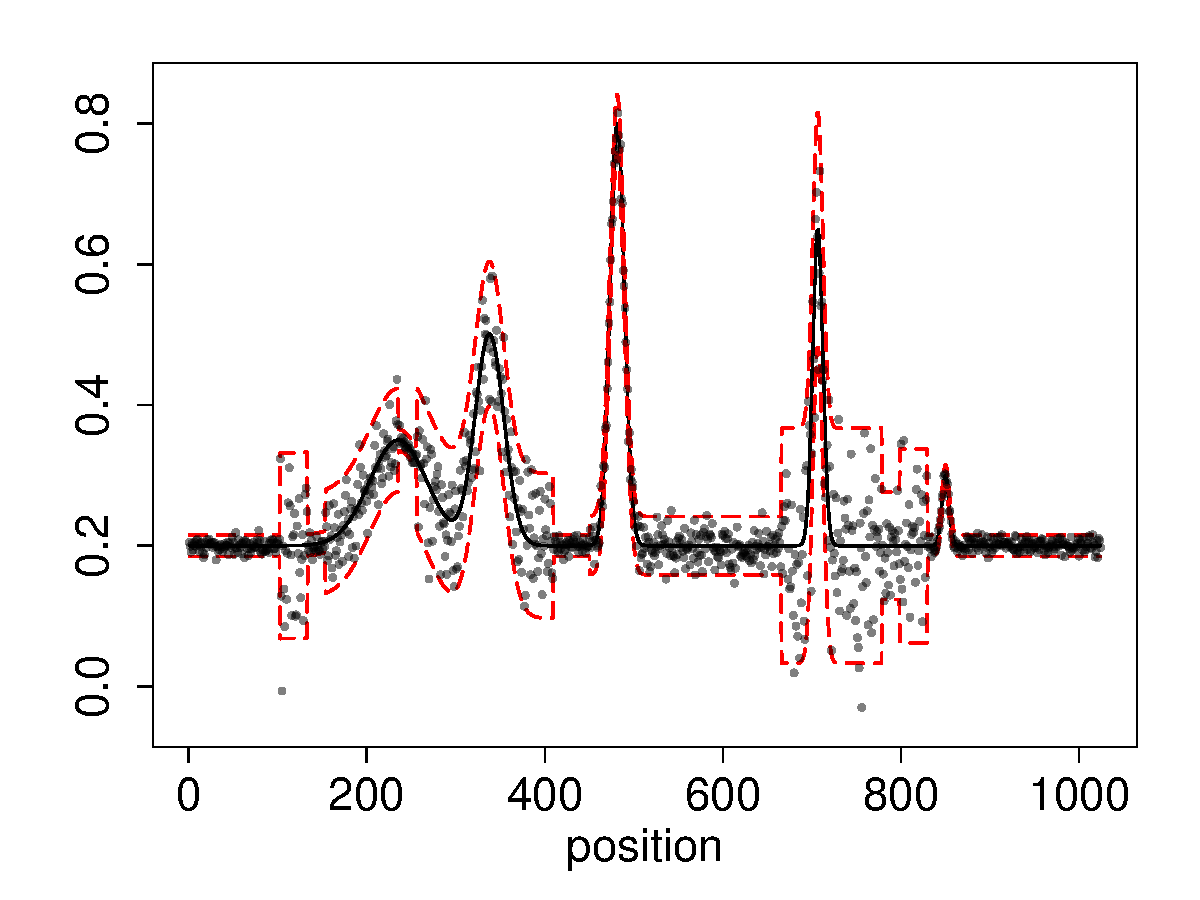
\includegraphics[width=\textwidth]{simple_eg_1.pdf}
        \caption{}
        \label{fig:simple_eg_1}
    \end{subfigure}
		\hfill
    \begin{subfigure}[b]{0.48\textwidth}
        \centering
        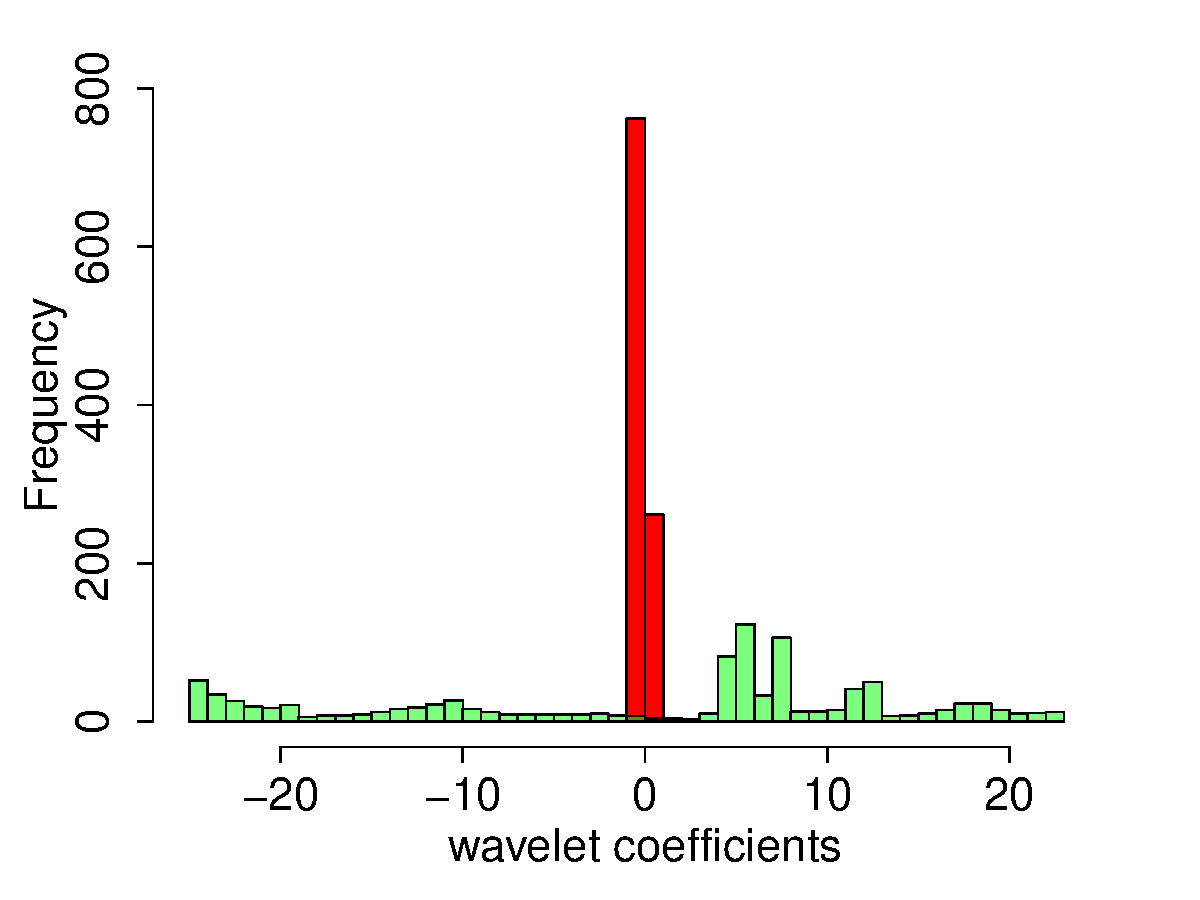
\includegraphics[width=\textwidth]{simple_eg_2.pdf}
        \caption{}
        \label{fig:simple_eg_2}
    \end{subfigure}
		\hfill
    \begin{subfigure}[b]{0.48\textwidth}
        \centering
        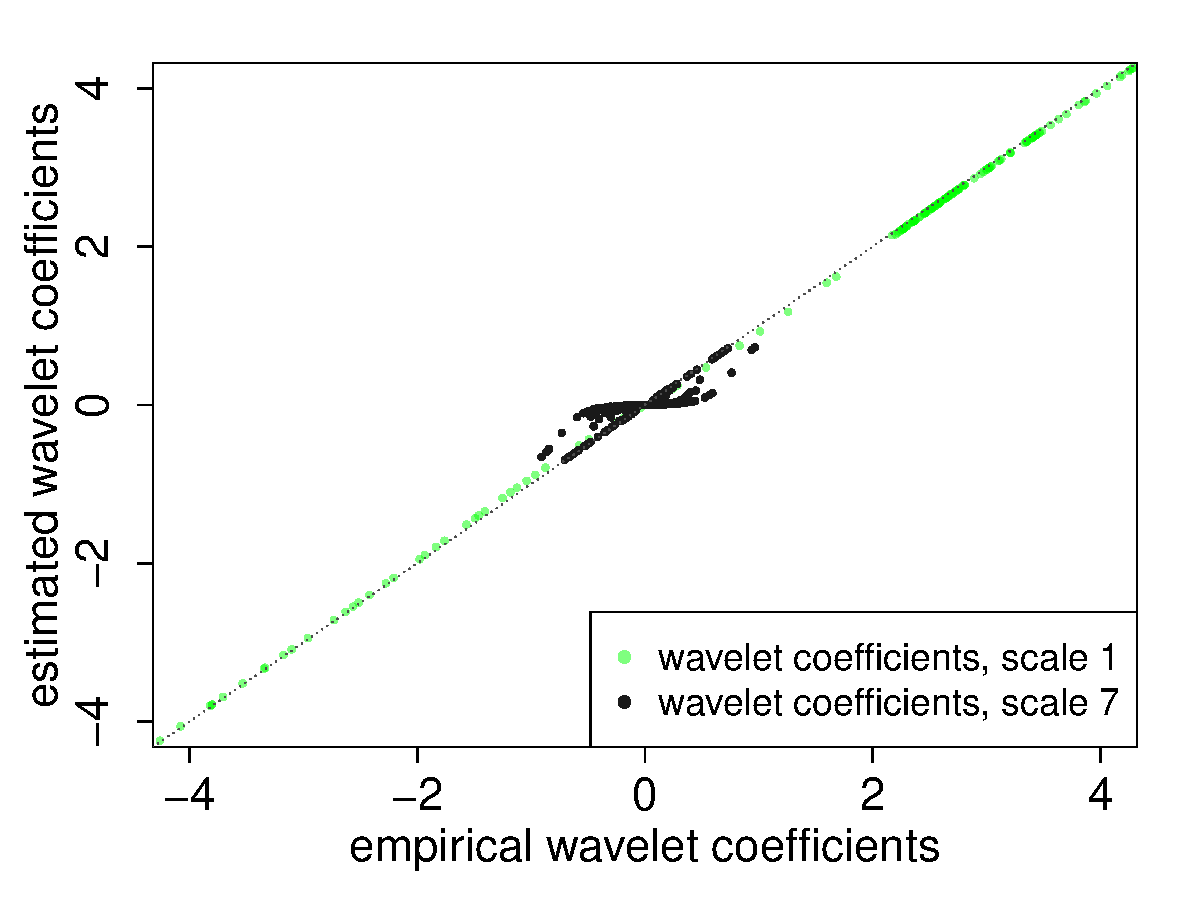
\includegraphics[width=\textwidth]{simple_eg_3.pdf}
        \caption{}
        \label{fig:simple_eg_3}
    \end{subfigure}
		\hfill
    \begin{subfigure}[b]{0.48\textwidth}
        \centering
        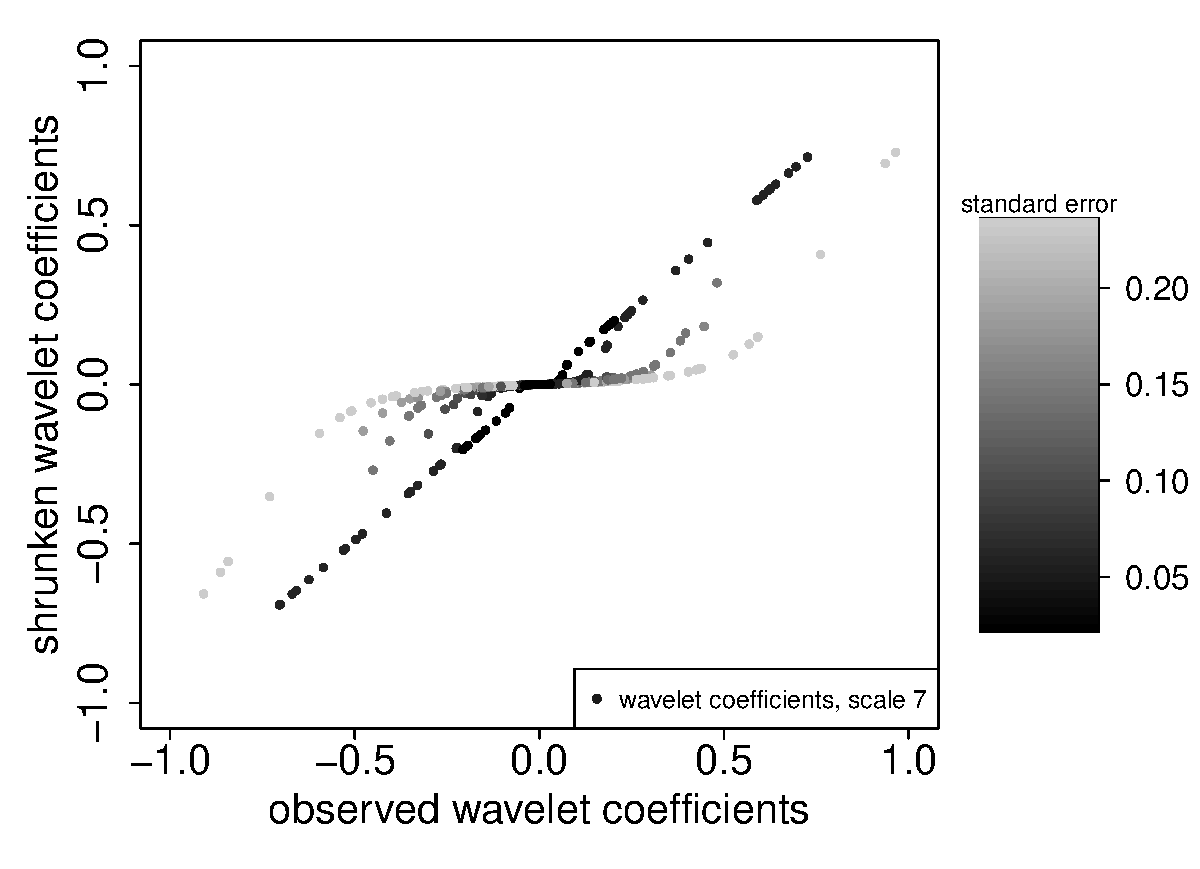
\includegraphics[width=\textwidth]{simple_eg_4.pdf}
        \caption{}
        \label{fig:simple_eg_4}
    \end{subfigure}
				\hfill
    \begin{subfigure}[b]{0.48\textwidth}
        \centering
        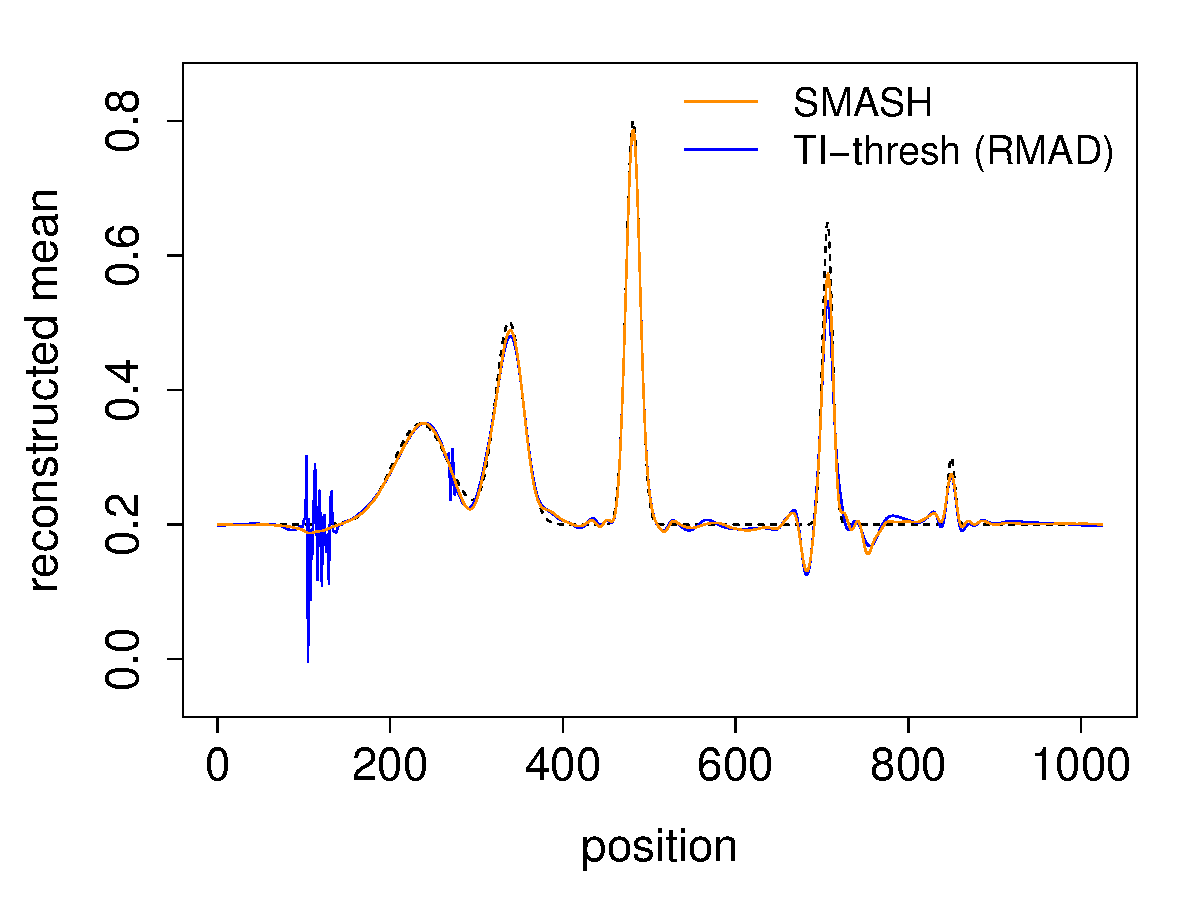
\includegraphics[width=\textwidth]{simple_eg_5.pdf}
        \caption{}
        \label{fig:simple_eg_5}
    \end{subfigure}
    \caption{Shows both ASH and SMASH at work. (a) shows the mean function $\pm$2 standard deviations, as well as one realized dataset. (b) contrasts the difference in the distribution of the true wavelet coefficients at two different scales - one coarse (scale 1) and one fine (scale 7). (c) demonstrates the shrinkage properties of ASH for the two scales of interest (scales 1 and 7): the coefficients at the fine scale (scale 7) are substantially shrunk, but barely so for the coarse scale. (d) shows the shrinkage effect of ASH on the fine scale (scale 7) wavelet coefficients - wavelet coefficients are shrunk adaptively based on their precision. (e) plots the estimated mean functions from SMASH and TI-thresh against the true mean function; we see that TI-thresh has noticeable artifacts.}
    \label{fig:simple_eg}
\end{figure}

\subsection{Simulations}

We conducted extensive simulation studies to compare the performance of our method with existing approaches.
 
 \subsubsection{Gaussian mean estimation}
 
For the Gaussian case, we focus on mean estimation, initially with homoskedastic errors. We modelled our simulation study after
\cite{Antoniadis2001Wavelet}, using many of the same test functions, a variety of sample sizes, two different signal to noise ratios (SNRs), and including
the best-performing methods from their comparison. In particular their results showed that Translation Invariant (TI) thresholding (\cite{Coifman1995Translationinvariant}) performed the best for most of the test signals, where performance is measured by mean squared error (MSE). We also considered the Empirical Bayes shrinkage procedure (\cite{Johnstone2005Empirical}), named Ebayesthresh. 
All the methods were applied using the Symmlet8 wavelet basis \cite{Daubechies1992Ten}.

Figure \ref{fig:gaus_homo} compares the mean integrated squared errors (MISEs) of TI-thresholding and Ebayesthresh to SMASH for the ``Spikes'' mean function, with a signal to noise ratio of 3 and sample size 1024. We applied SMASH in three ways, the first (SMASH) estimating the variance function allowing for heteroskedasticity, the second estimating the variance assuming homoskedasticity (SMASH-homo) and the
third using the true variance function (SMASH true variance), which could be viewed as a "gold standard". The results show that all three versions of SMASH outperform both EbayesThresh and TI-thresholding. Notably all three SMASH versions perform very similarly, demonstrating that
in this case there is little cost in allowing for heterskedasticity when the truth is homoskedastic.

We obtained similar results for other mean functions, SNRs and sample sizes (see Supplementary Materials).

\begin{figure}
\centering
    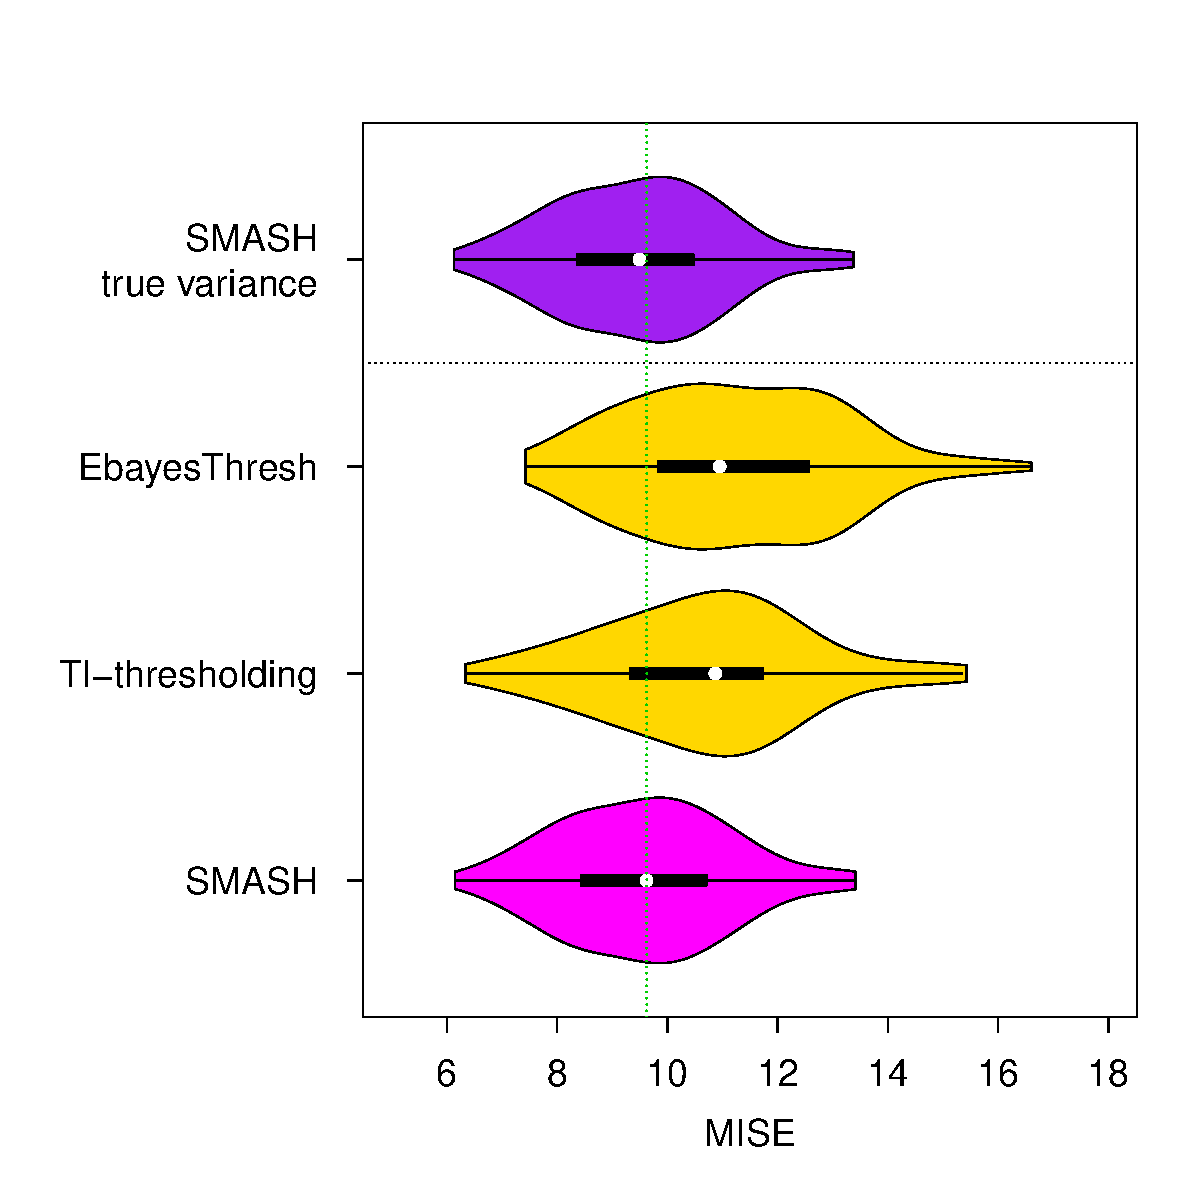
\includegraphics[width=0.65\textwidth]{violin_gaus_homo.pdf}
    \caption{Comparison of wavelet-based methods for mean estimation with homoskedastic Gaussian errors for the ``Spikes'' mean function. Violin plots of MISEs for (from bottom to top) SMASH, SMASH with homoskedastic assumption, TI-thresholding with homoskedastic assumption, Ebayesthresh with homoskedastic assumption, and SMASH with known true variance are shown in the figure. Smaller MISE implies better performance; dashed green line indicates the median MISE for SMASH. SMASH outperforms both TI-thresholding and Ebayesthresh, and SMASH with estimated variance performs nearly as well as with true variance.}
    \label{fig:gaus_homo}
\end{figure}

Turning now to heteroskedastic errors, we compare results from SMASH (run three different ways, as above) with EbayesThresh (which assumes
homoskedastic variance) and TI-thresh. For TI-thresh we considered three different ways of estimating the heteroskedastic variance: RMAD 
(\cite{Gao1997Wavelet}), the SMASH estimated variance, and the true variance. (TI-thresh with homoskedastic variance performed very poorly; Supplementary Results.) Figure \ref{fig:gaus_hetero} 
shows results for two sets of test functions: the ``Spikes'' mean function with the ``Clipped Blocks'' variance function and the ``Corner'' mean function with ``Doppler'' variance function, both with SNRs of 3 and sample sizes of 1024. 

To summarize the main patterns in Figure \ref{fig:gaus_hetero}:
\begin{enumerate}
\item SMASH outperforms all TI-thresh variants (including, here, TI with the true variance).
\item SMASH performs almost as well for mean estimation when estimating the variance as when given the true variance.
\item Allowing for heteroskedasticity within SMASH can substantially improve accuracy of mean estimation (compare SMASH with SMASH-homo and EbayesThresh).
\item TI-thresh performs considerably better when used with the SMASH variance estimate than with the RMAD variance estimate.
\end{enumerate}

These main patterns hold for a variety of different mean and variance functions, SNRs, and sample sizes (see Supplementary Materials). Some variance functions are harder to estimate than others (e.g. the ``Bumps" function), and in these cases providing methods the true variance can greatly increase
accuracy compared with estimating the variance. 
As might be expected, the gain in allowing for heteroskedastic variance tends to be greatest when the variance functions are more
volatile.

\begin{figure}
\centering
    \begin{subfigure}[b]{0.65\textwidth}
        \centering
        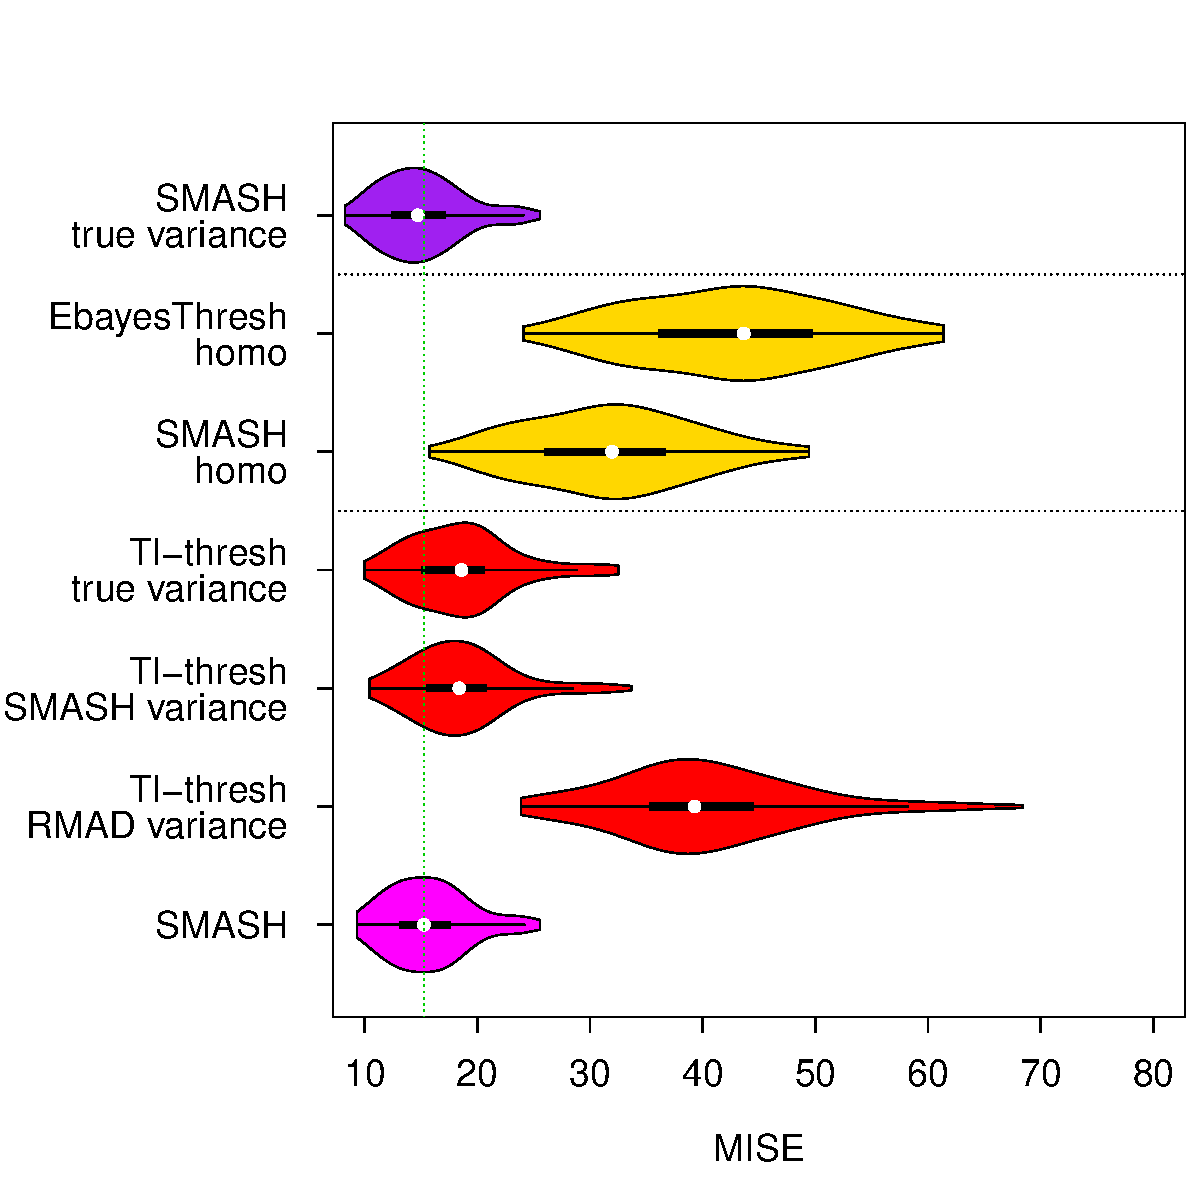
\includegraphics[width=\textwidth]{violin_gaus_hetero_1.pdf}
        \caption{}
        \label{fig:gaus_hetero_1}
    \end{subfigure}
		\hfill
    \begin{subfigure}[b]{0.3\textwidth}
        \centering
        \raisebox{0.5\height}{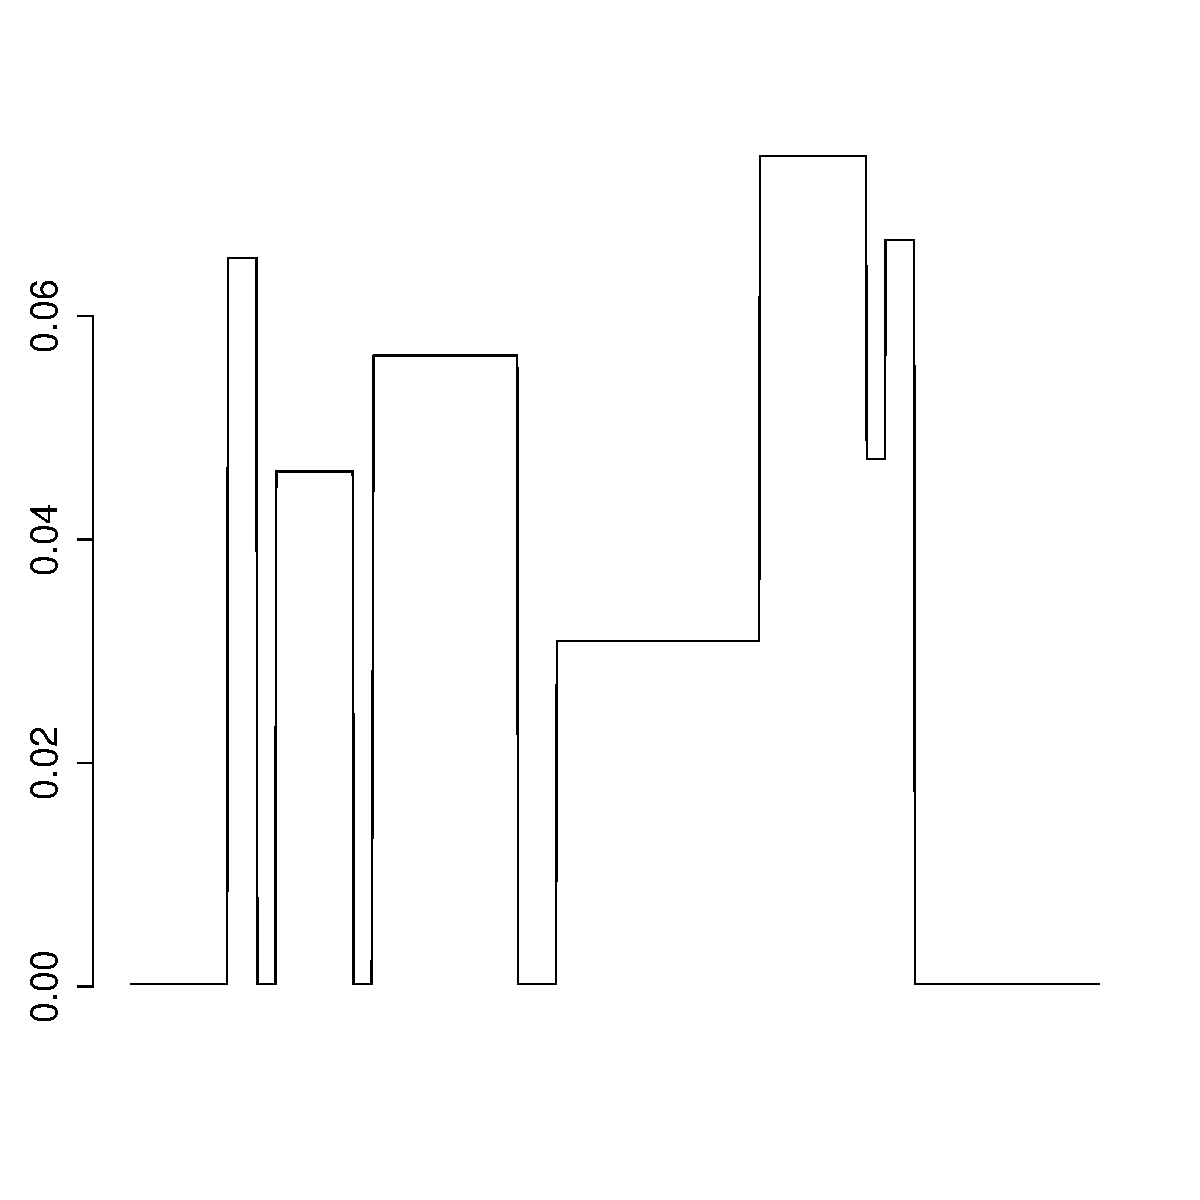
\includegraphics[width=\textwidth]{violin_gaus_hetero_sd_1.pdf}}
        \caption{}
        \label{fig:gaus_hetero_sd_1}
    \end{subfigure}
		\hfill
    \begin{subfigure}[b]{0.65\textwidth}
        \centering
        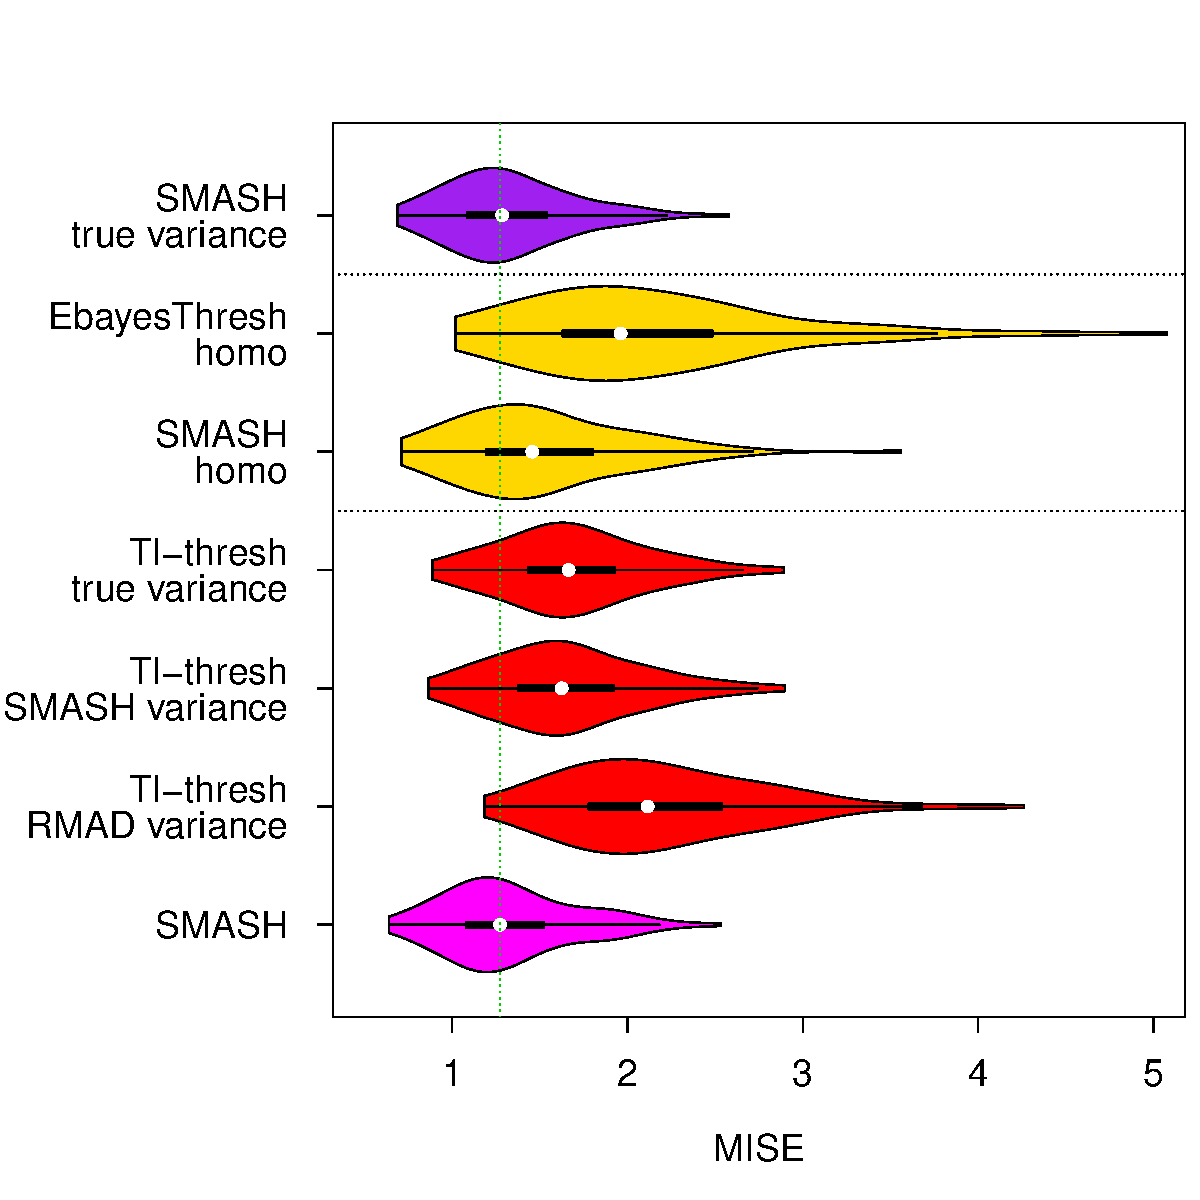
\includegraphics[width=\textwidth]{violin_gaus_hetero_2.pdf}
        \caption{}
        \label{fig:gaus_hetero_2}
    \end{subfigure}
		\hfill
    \begin{subfigure}[b]{0.3\textwidth}
        \centering
        \raisebox{0.5\height}{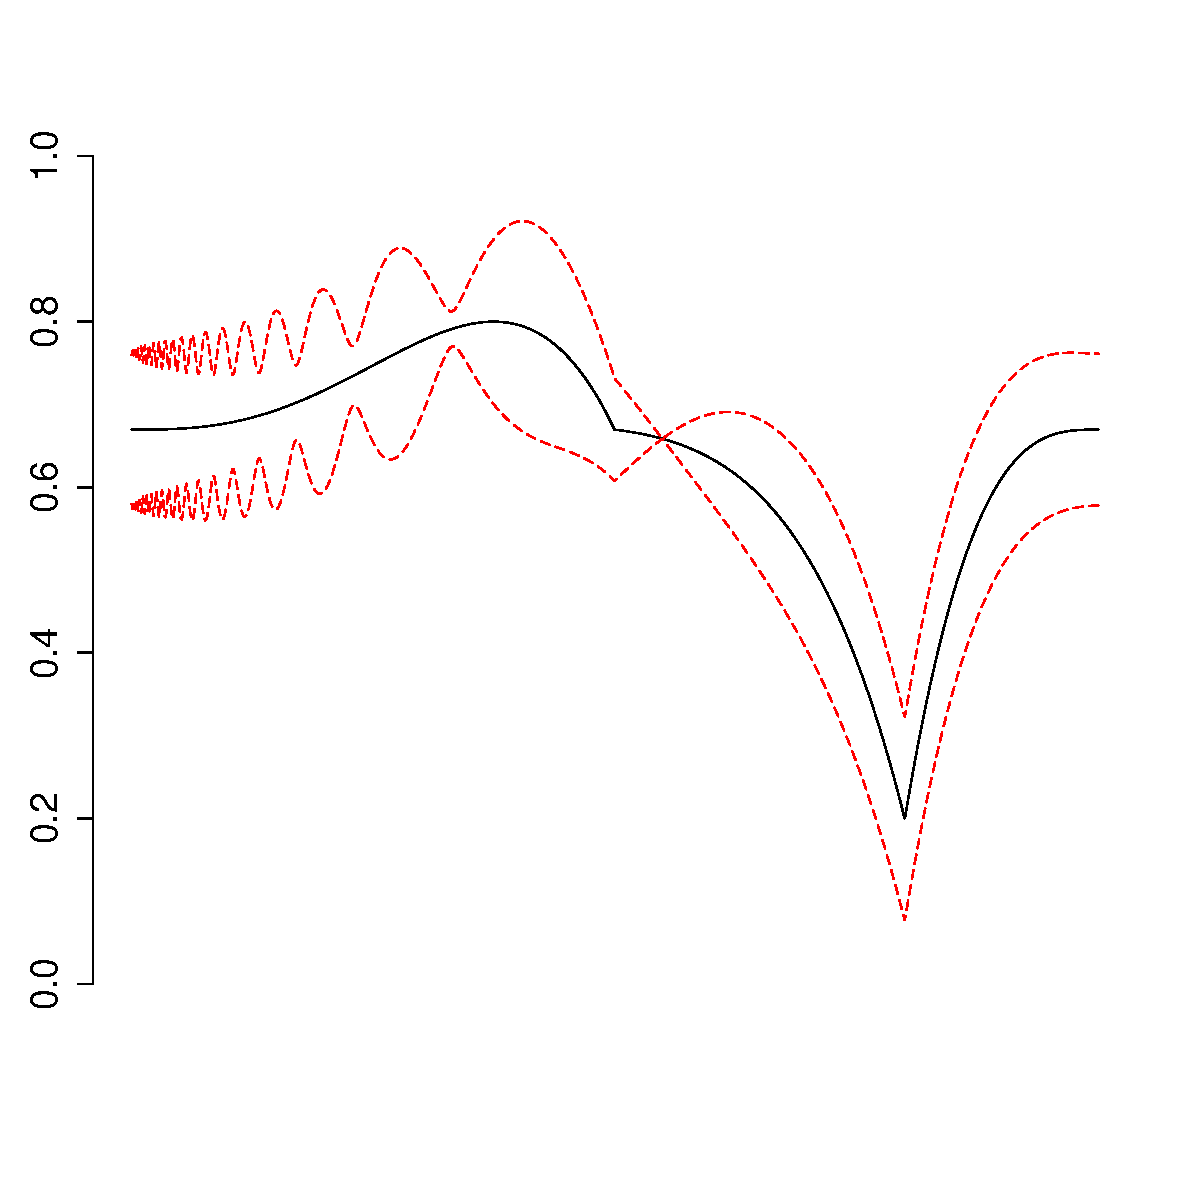
\includegraphics[width=\textwidth]{violin_gaus_hetero_sd_2.pdf}}
        \caption{}
        \label{fig:gaus_hetero_sd_2}
    \end{subfigure}
    \caption{Comparison of wavelet-based methods for mean estimation with heteroskedastic Gaussian errors. Figures on the left show violin plots of MISEs for various methods on two sets of mean-variance functions: ``Spikes'' mean function with ``Clipped Blocks'' variance function, and ``Corner'' mean function with ``Doppler'' variance function. Smaller MISE implies better performance; dashed green line indicates the median MISE for SMASH. Figures on the right plot the mean functions $\pm$2 standard deviations.}
    \label{fig:gaus_hetero}
\end{figure}


\subsubsection{Gaussian variance estimation}\label{sec:mfvb}

One unusual feature of SMASH is that it performs joint mean and variance estimation.
Indeed, we found no existing R packages aimed at doing this. However we were able to obtain code
implementing the Mean Field Variational Bayes (MFVB) method for heteroskedastic Gaussian regression \cite{Menictas2015Variational} (M.~Menictas, personal communication). 
This method is based on penalized splines, and so is not well suited to many standard test functions in the wavelet literature, which
often contain ``spiky" local features not well captured by splines. Hence, we compared SMASH and MFVB on some
smoother mean and variance (standard deviation) functions, specifically scenario A in Figure 5 from \cite{Menictas2015Variational} (Figure \ref{fig:mfvb_eg}),
using scripts kindly provided by M.~Menictas.

We simulated data under two different scenarios:
\begin{enumerate}
\item We generated $n=500$ independent $(X_i,Y_i)$ pairs, with $X_i \sim$ Uniform(0,1), and $Y_i | X_i=x_i \sim N(m(x_i),s(x_i)^2)$
where $m(\cdot)$ and $s(\cdot)$ denote the mean and standard deviation functions (Figure \ref{fig:mfvb_eg}). We measured performance by the MSE 
evaluated at 201 equally spaced points on $(X_{min},X_{max})$ for both the mean and the standard deviation.
\item We generated $n=1024$ independent $(X_i,Y_i)$ pairs, with the $X_i$'s (deterministically) equally spaced on (0,1), and $Y_i|X_i$ as above. Performance is measured by MSE evaluated at the 1024 $X_i$'s for both the mean and the standard deviation.
\end{enumerate}
\begin{figure}[ht]
    \centering
    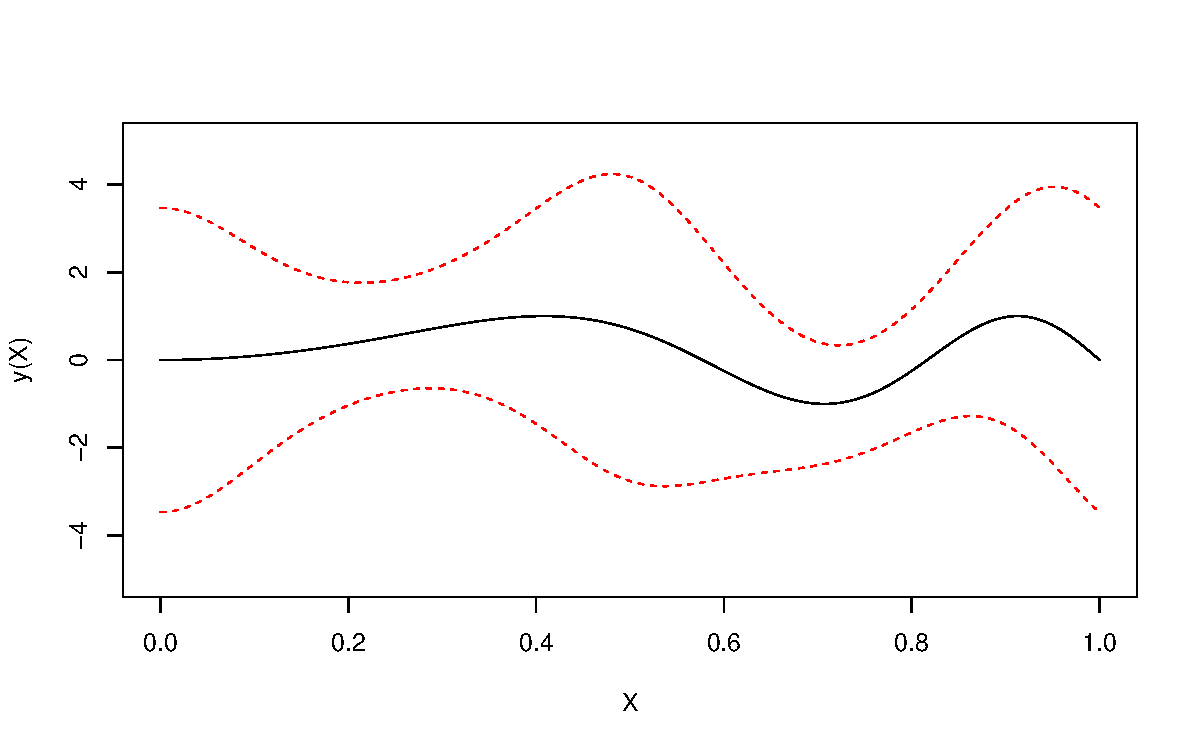
\includegraphics[width=\textwidth]{mfvb_eg.pdf}
    \caption{Shows the mean function $m(x)$ $\pm$2 standard deviations $s(x)$ used in the simulation study comparing SMASH against MFVB. These functions correspond to mean and standard deviation functions (A) in Figure 5 from \cite{Menictas2015Variational}.}
    \label{fig:mfvb_eg}
\end{figure}

The first scenario presents some issues for SMASH because the number of data points is not a power of two, nor are the points equally-spaced. To deal with the first issue, following standard ideas in the wavelet literature, we first mirrored the data about the right edge and extract the first $2^{\lfloor\log_2(2n)\rfloor}$ sample points, so that the number of data points in the new ``dataset'' is a power of two, and the mean curve is continuous at the right edge. To further ensure that the input to SMASH is periodic, we reflected the new dataset about the right edge and used this as the final input. 
To deal with the second issue we follow the common practice of treating the observations as if they are evenly spaced (see \cite{Sardy1999Wavelet} for discussion). To estimate the original mean and variance functions, we extract the first $n$ points from the SMASH estimated mean and variance. 
To evaluate MSE at the 201 equally spaced points (Scenario 1) we use simple linear interpolation between the estimated points. 

Table \ref{table:mfvb_comp} shows mean MSEs over 100 independent runs for each scenario.
Despite the fact that these simulation scenarios -- particularly Scenario 1 -- seem better suited to MFVB than SMASH, 
SMASH performs comparably or better than MFVB for both mean and variance estimation in both Scenarios. 
\begin{table}[ht]
\centering
\begin{tabular}{rrrrr}
\hline
& \multicolumn{2}{c}{Scenario 1}&\multicolumn{2}{c}{Scenario 2}\\
\cline{2-5}
& MSE (for mean) & MSE (for sd) & MSE (for mean) & MSE (for sd) \\
\hline
MFVB & 0.0330 & 0.0199 & 0.0172 & 0.0085 \\
SMASH & 0.0334 & 0.0187 & 0.0158 & 0.0065 \\
\hline
\end{tabular}
\caption{Comparison of accuracy (MSE) of SMASH and MFVB for two simulation scenarios.  True mean and sd functions are shown in \ref{fig:mfvb_fn}. 
In Scenario 1 the data are not equally spaced and not a power of 2; here SMASH is comparable to MFVB in mean estimation and more accurate for sd estimation.
In Scenario 2 the data are equally spaced and a power of 2; here SMASH outperforms MFVB in both mean and sd estimation.}
\label{table:mfvb_comp}
\end{table}

 

\subsubsection{Poisson Data}

To assess SMASH on Poisson data we simulated data from
several different test functions from \cite{Timmermann1999Multiscale}, \cite{Fryzlewicz2004HaarFisz} and \cite{Besbeas2004Comparative}.
We varied the minimum and maximum intensity of each test function, using (min,max) intensities of (0.01,3), (1/8,8) and (1/128,128).
For each test function and intensity level we simulated 100 datasets, each with $n=1024$ data points.
We focus on results for the first two intensity settings, which have smaller average intensity. These settings produce smaller average counts, making them more challenging, and also more representative of the kinds of genomic application that we consider below.
Complete results are included in Supplementary Materials.

We compared SMASH with six other methods, but we focus here on the comparisons with the best-performing other methods, which are Haar-Fisz (HF) (\cite{Fryzlewicz2004HaarFisz}) and BMSM (\cite{Kolaczyk1999Bayesian}). The latter, like SMASH, is an Empirical Bayes method,  but with a less flexible prior distribution on the
multi-scale coefficients. The HF method involves first performing a transformation on the Poisson counts, and applying Gaussian wavelet methods to the transformed data. 
There are many choices for Gaussian wavelet methods, and the performance depends on these choices (and with different choices being optimal for different data sets). 
The settings we used here are documented in Supplementary Information, and were chosen by us to optimize (average) performance through moderately extensive experimentation on a range of simulations.

In summary, SMASH outperformed both HF and BMSM in the majority of simulations, with the gain in accuracy being strongest for the more challenging lower-intensity
scenarios. A typical result is shown in Figure \ref{fig:pois_sim}, with complete results in Supplementary Information. 
Among the other two methods, BMSM tends to be the more consistent performer. HF, with the settings
we used here, performs quite variably, being worse than the other two in most scenarios, but occasionally performing the best (specifically for the Angles, Bursts and Spikes test functions,
with (min,max) intensity (1/128,128)). As noted above, the HF transform can be used with many settings, so the results here should be viewed as a guide to the 
performance that can be achieved in practice.


%Besides the somewhat strong assumption of unit variance, the inconsistent performance of Haar-Fisz could also be attributed to the choice of the primary resolution level used, which can substantially affect the performance of Haar-Fisz. Here we analyzed primary resolution levels of 4, 5, 6 and 7, similar to \cite{Besbeas2004Comparative}. On the other hand, SMASH outperforms BMSM consistently, even though it is based on the same likelihood factorization used in the latter. We can thus conclude that the choice of ASH as the shrinkage procedure is superior to that used in BMSM in the simulation study. More importantly, using this formulation in SMASH also makes it easily extensible to multiple samples in the context of a (generalized) linear model, something we will briefly describe in the Discussion section.
\begin{figure}
\centering
		\begin{subfigure}[b]{0.75\textwidth}
        \centering
        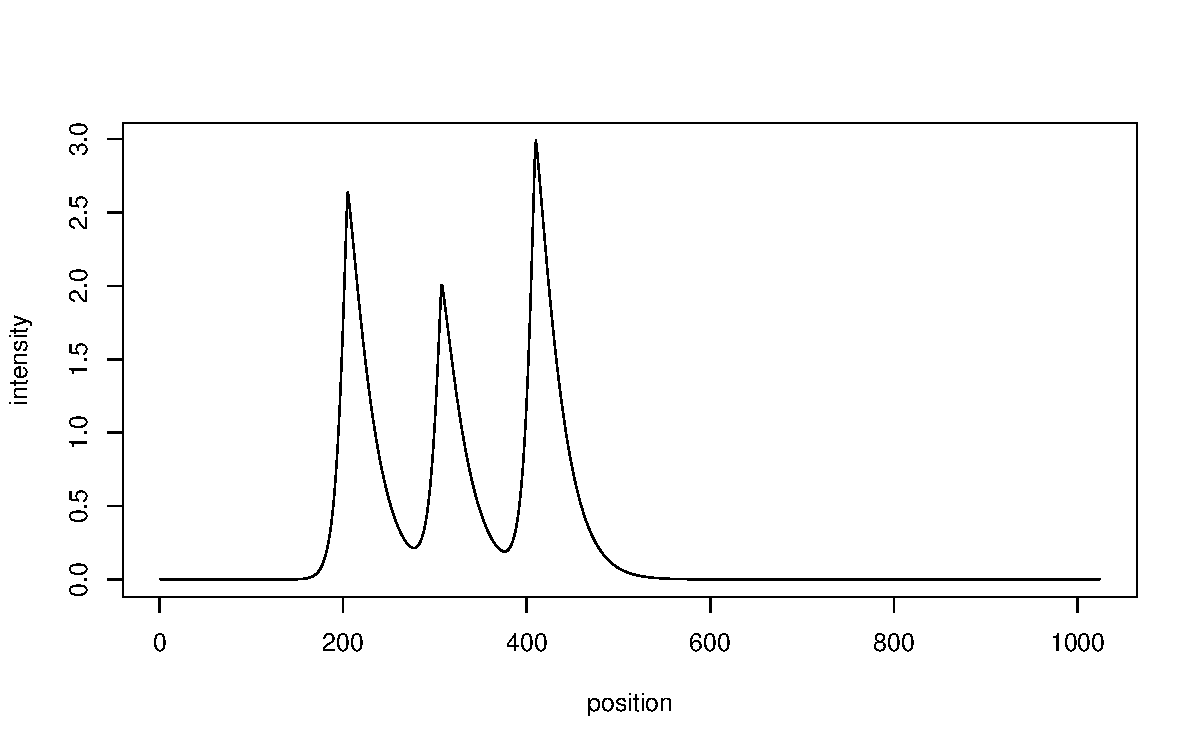
\includegraphics[width=\textwidth]{bursts_pois.pdf}
        \caption{}
        \label{fig:bursts_fn}
    \end{subfigure}
    \begin{subfigure}[b]{0.45\textwidth}
        \centering
        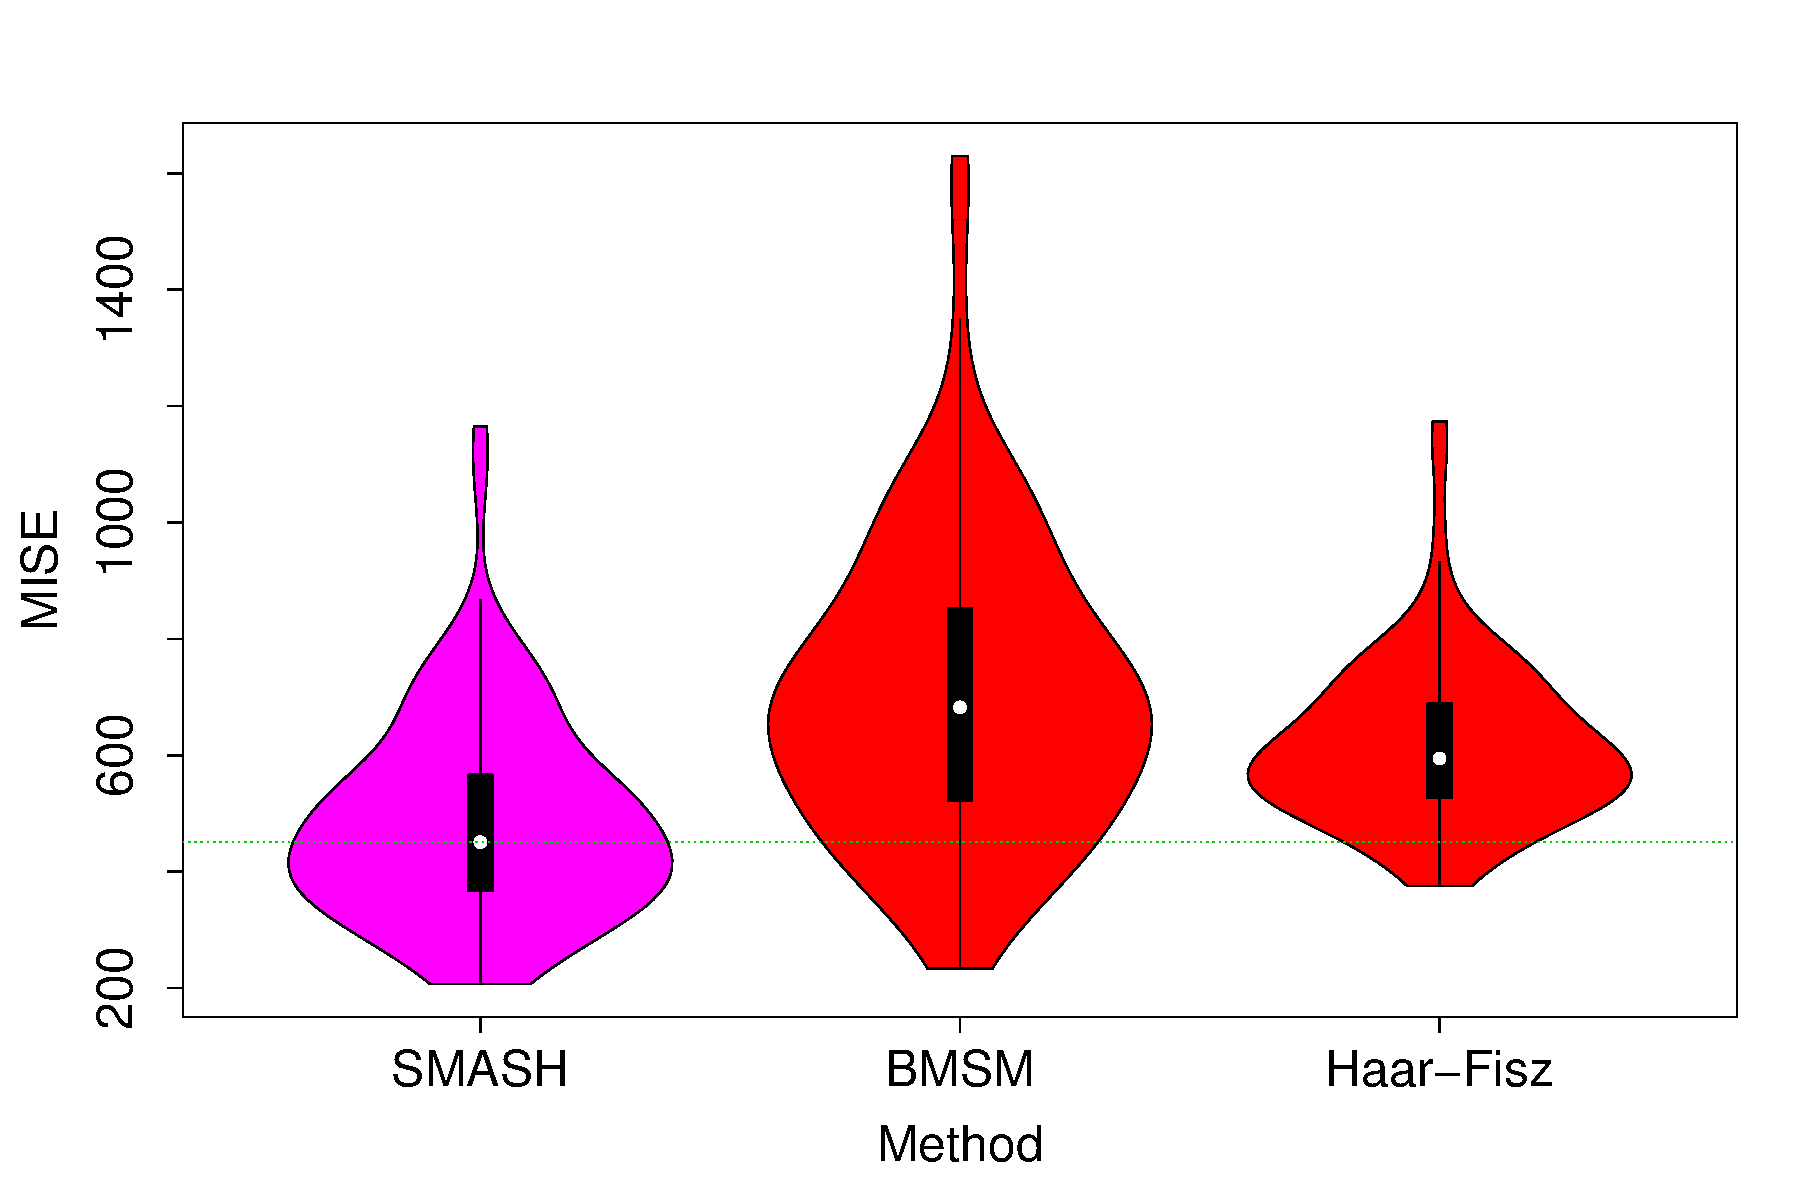
\includegraphics[width=\textwidth]{violin_pois_1.pdf}
        \caption{}
        \label{fig:pois_1}
    \end{subfigure}
		\hfill
    \begin{subfigure}[b]{0.45\textwidth}
        \centering
        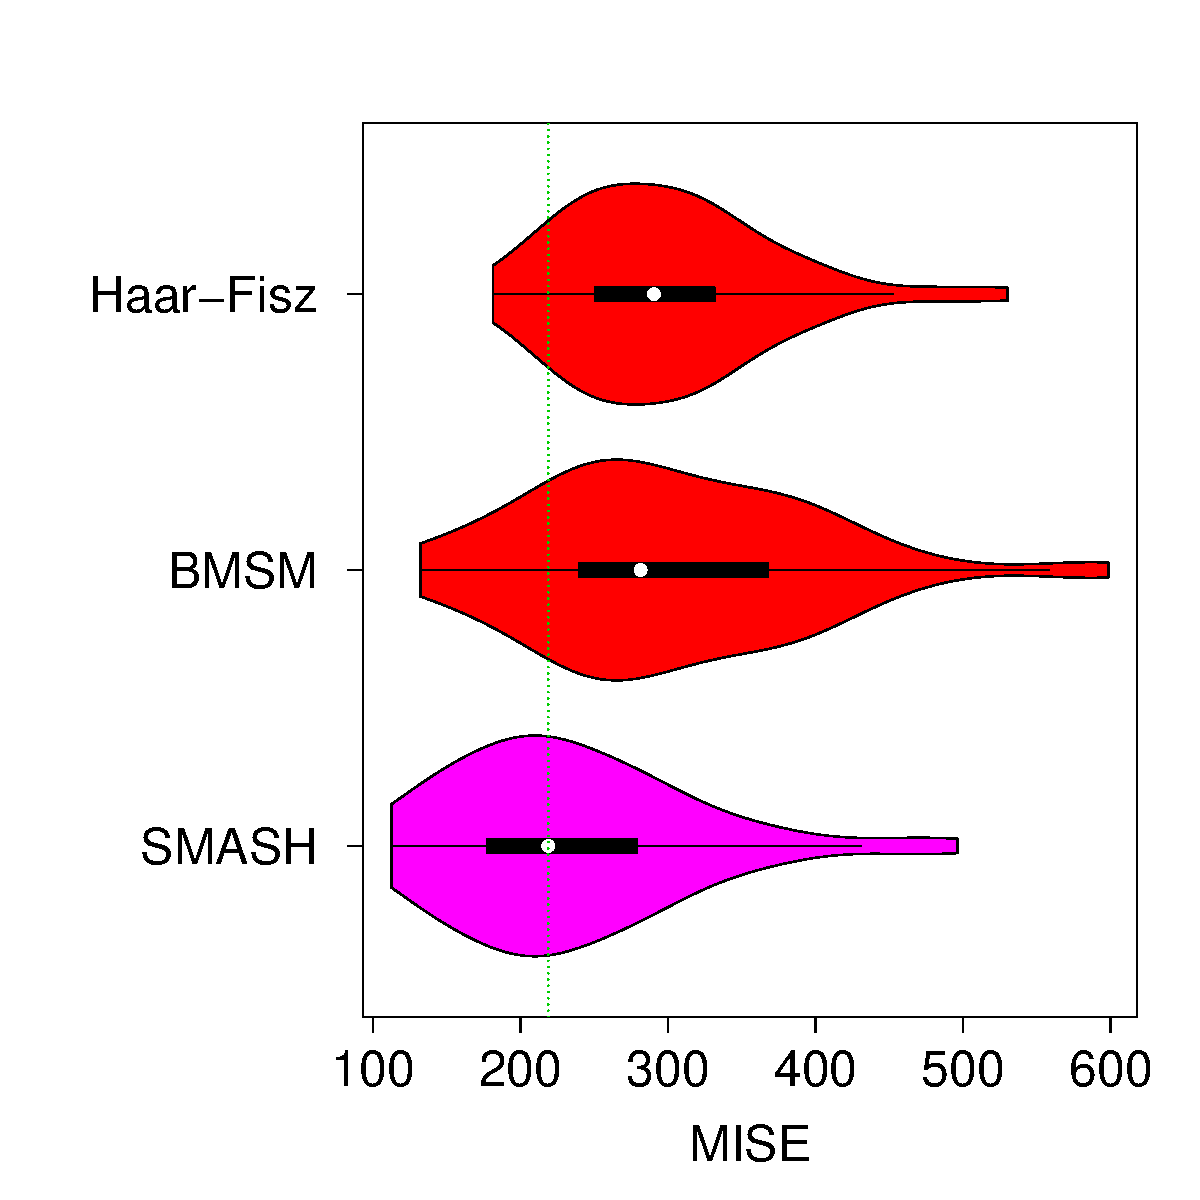
\includegraphics[width=\textwidth]{violin_pois_8.pdf}
        \caption{}
        \label{fig:pois_8}
    \end{subfigure}
    \caption{Comparison of methods for denoising Poisson data for the ``Bursts'' test function. (a) shows the (unscaled) test function. The violin plots in (b) and (c) show distributions of MISE for each method over 100 datsets, with smaller values indicating better performance. The dashed green line indicates the median MISE for SMASH. Panel (b) corresponds to a (min,max) intensity of (0.01,3), and (c) corresponds to a (min,max) intensity of (1/8,8).}
    \label{fig:pois_sim}
\end{figure}

One disadvantage of the HF transform is that, to achieve translation invariance (TI), the transform has to be done explicitly for each shift of the data: the tricks usually used to do this efficiently \cite{Coifman1995Translationinvariant} do not work here. Thus, making HF fully translation invariant increases computation by a factor of $T$, rather than the factor of $\log(T)$ for the other methods. Here we follow advice in \cite{Fryzlewicz2004HaarFisz} to reduce the computational burden by averaging over 50 shifts of the data rather than $T$. Even so, HF was substantially slower than the other methods.
 A direct comparison of computational efficiency between SMASH and BMSM is difficult, as they are coded in different programming environments. Nevertheless, similarities between the two methods suggest that they should have similar computational cost.
 Both SMASH and BMSM took, typically, less than a second per dataset in our simulations.

%Overall, these simulation studies demonstrate the ability of SMASH to accurately recover the mean functions for both the Gaussian and Poisson cases, and highlight the flexibility and adaptivity of the shrinkage procedure ASH. Although we have considered an extensive range of scenarios here, including different SNRs, sample sizes, variance functions, test functions and mean intensities where applicable, the performance of our method on real data has yet to be determined. In the next section, we will apply our method to two example datasets that have been discussed in previous work, and comment on the resulting estimates.


\section{Illustrative applications}
%\subsection{Three-month Treasury Bill Yields}
%In this section we apply the Gaussian and Poisson denoising techniques to one example dataset each. For the Gaussian case, we looked at yields of secondary market rates from three-month Treasure bills, which were recorded weekly on Fridays. These rates were quoted on a discount basis and annualized using a 360-day year of bank interest. To match the analysis in \cite{Fan1998Efficient}, we used 1735 weekly observations spanning Jan. 5 1962 to Mar. 31 1995. The data are plotted in Figure \ref{fig:tb_raw_data}. Similar to \cite{Fan1998Efficient}, we fit an autoregressive model of order 5 (AR(5)) to the data and obtained the following:
%\begin{eqnarray}
%T_t=1.228T_{t-1}-0.234T_{t-2}+0.028T_{t-3}+0.039T_{t-4}-0.066T_{t-5}+Y_t
%\end{eqnarray}
%where $T_t, t=1,...,1735$ is the time series for the yields, and $Y_t$ are the residuals from fitting the model. Figure \ref{fig:tb_res} shows the plot of $Y_t$ against $X_t\equiv T_{t-1}$. Our goal is to estimate the mean function defined by $E(Y_t|X_t=x)$ as well as the variance function $V(Y_t|X_t=x)$. Note that standard wavelet techniques are not designed for such types of data, where 1) repeated observations are present and 2) the number of data points is not a power of two and the points are unevenly spaced. To tackle the first issue, we use the median of the repeated observations at their respective sample points (see eg \cite{Delouille2004Smooth}). Next, we applied the procedure described in the Simulations section when comparing our method against MFVB, which was a modified version of symmetric extension. This deals with the second complication. The estimated mean and variance functions are given in Figures \ref{fig:tb_res} and \ref{fig:tb_var} respectively.
%
%\begin{figure}
%\centering
    %\begin{subfigure}[b]{0.4\textwidth}
        %\centering
        %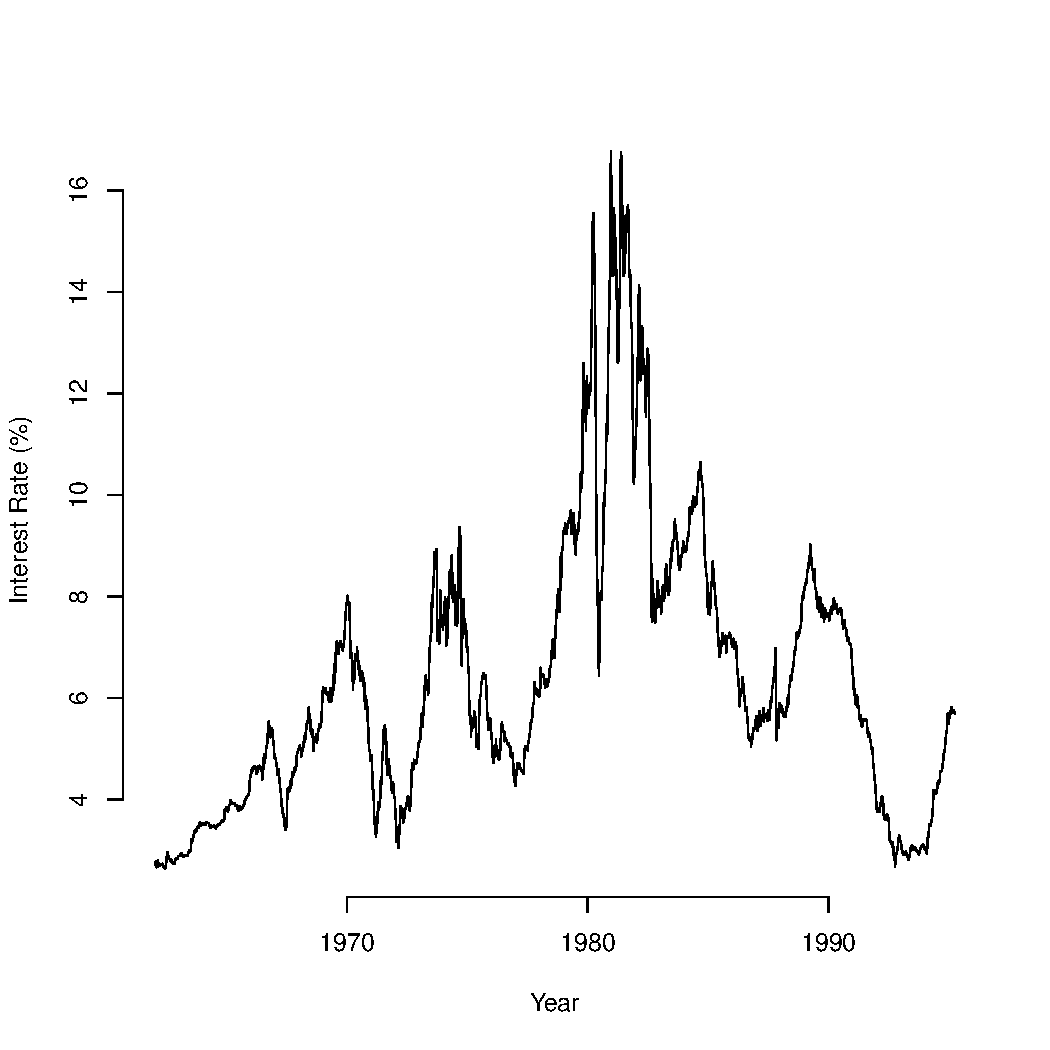
\includegraphics[width=\textwidth]{figures_treasury_a.pdf}
        %\caption{}
        %\label{fig:tb_raw_data}
    %\end{subfigure}
    %\hfill
    %\begin{subfigure}[b]{0.4\textwidth}
        %\centering
        %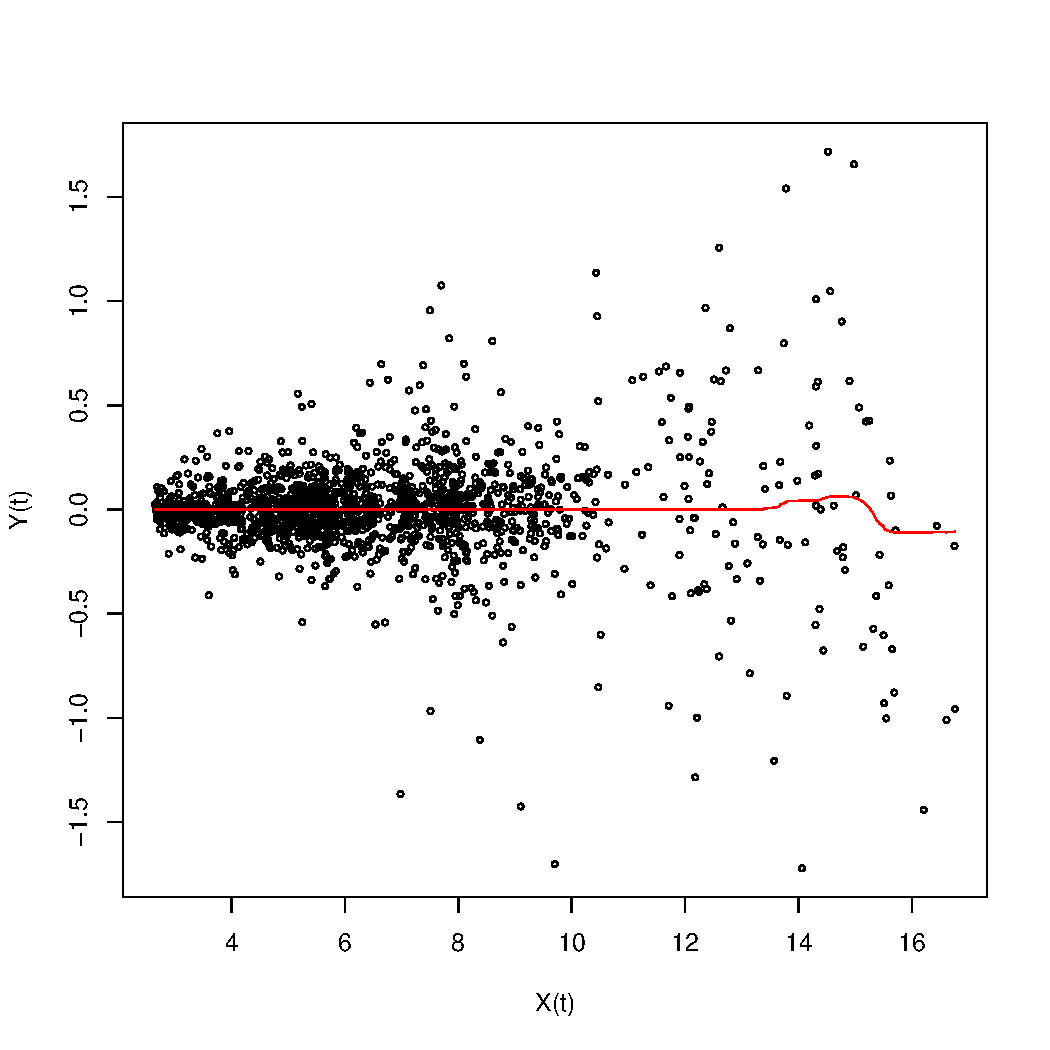
\includegraphics[width=\textwidth]{figures_treasury_b.pdf}
        %\caption{}
        %\label{fig:tb_res}
    %\end{subfigure}
    %\begin{subfigure}[b]{0.4\textwidth}
        %\centering
        %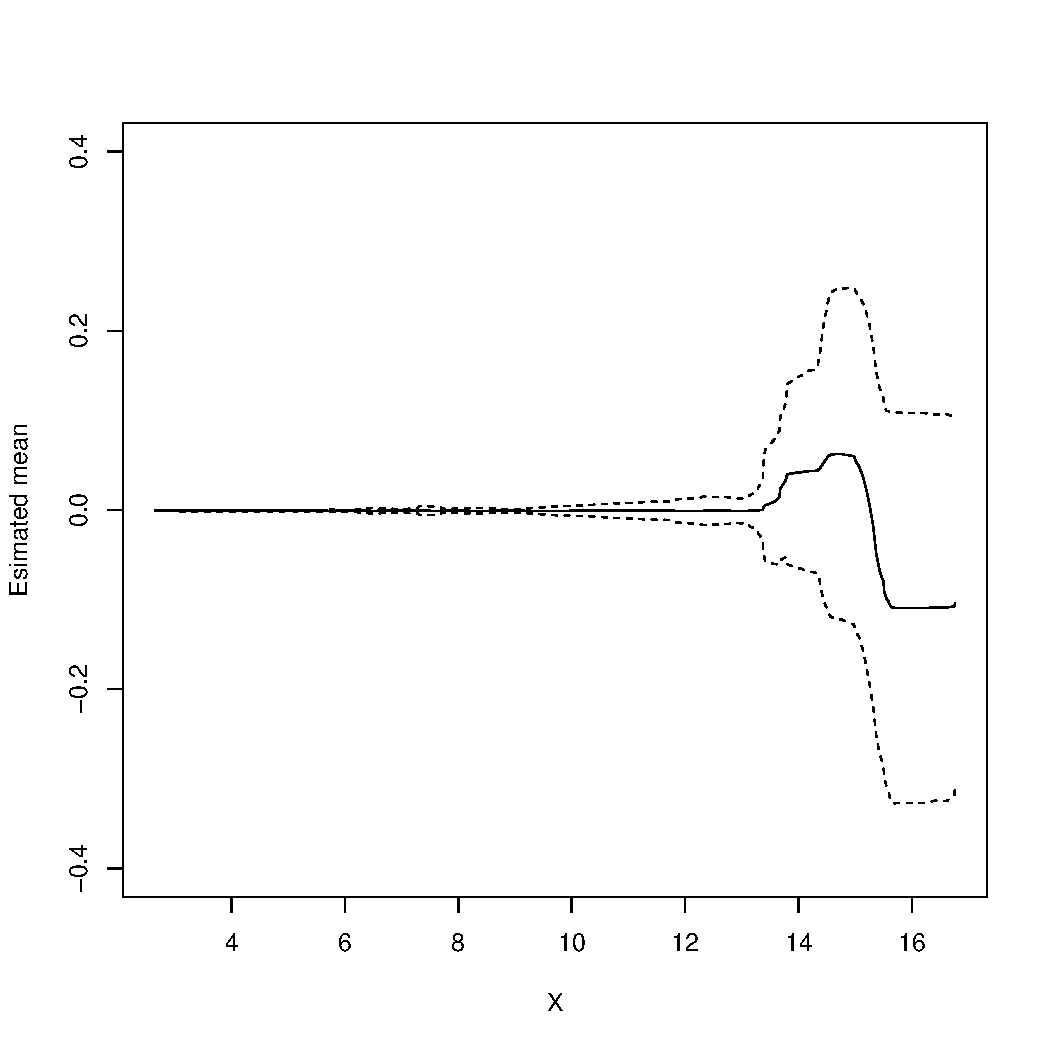
\includegraphics[width=\textwidth]{figures_treasury_c.pdf}
        %\caption{}
        %\label{fig:tb_mean}
    %\end{subfigure}
    %\hfill
    %\begin{subfigure}[b]{0.4\textwidth}
        %\centering
        %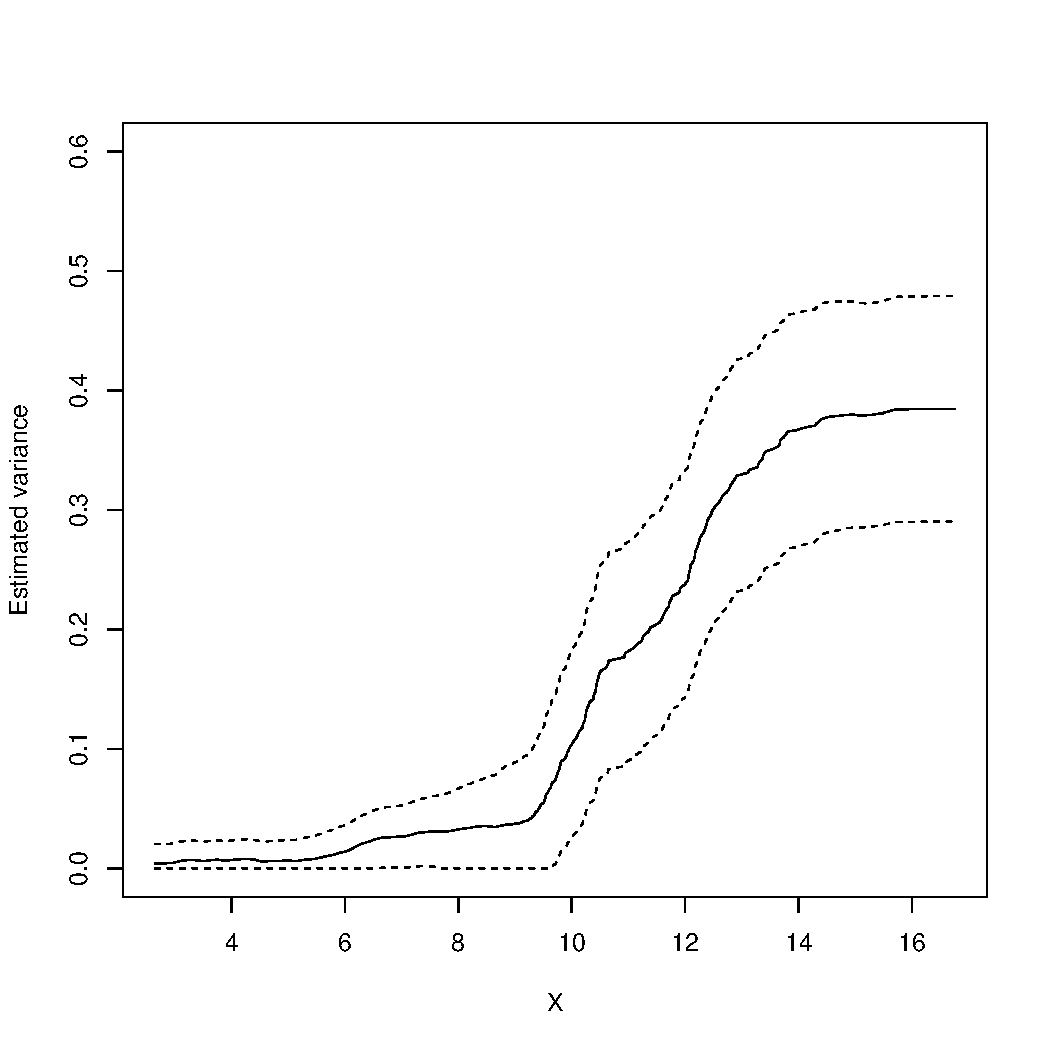
\includegraphics[width=\textwidth]{figures_treasury_d.pdf}
        %\caption{}
        %\label{fig:tb_var}
    %\end{subfigure}
    %\caption{Analysis of yields from three-month Treasury Bills. (a) Raw data of interest rates as a function of time. (b) Residuals $Y_t$ from fitting an AR(5) model to the data against $X_t\equiv T_{t-1}$. The red curve is the estimated mean curve from SMASH. (c) Plot of a zoomed-in version of the estimated mean curve, with approximate 95\% credible bands. (d) The estimated conditional variance curve, with approximate 95\% credible bands.}
%\end{figure}
%
%Except for possible boundary effects, our mean and conditional variance estimates are similar to those of \cite{Fan1998Efficient}. Unfortunately, these boundary effects are difficult to deal with for non-periodic functions in the wavelet case, and our usage of symmetric extension with the Haar basis is just one possible solution. Better alternatives have been suggested by eg. Su et al. (2013), but is beyond the scope of discussion in this paper. Similar to the analysis in \cite{Fan1998Efficient}, we found the correlation coefficient between the logarithm of $x_t$ and the logarithm $\hat{V}^{1/2}(Y_t|x_t)$ to be 0.949, which further supports the structural volatility model suggested by Andersen and Lund (source?):
%\begin{eqnarray}
%Var^{1/2}(Y_t|x_t)=\Ga x_t^{\Gb}
%\end{eqnarray}
%By performing least squares regression of $\log(\hat{V}^{1/2}(Y_t|x_t))$ on $\log(x_t)$, we have that $\hat{\Ga}=0.0106$ and $\hat{\Gb}=1.429$, which are similar to the values reported in \cite{Fan1998Efficient}.
\subsection{Motorcycle Acceleration Data}
\begin{figure}
\centering
    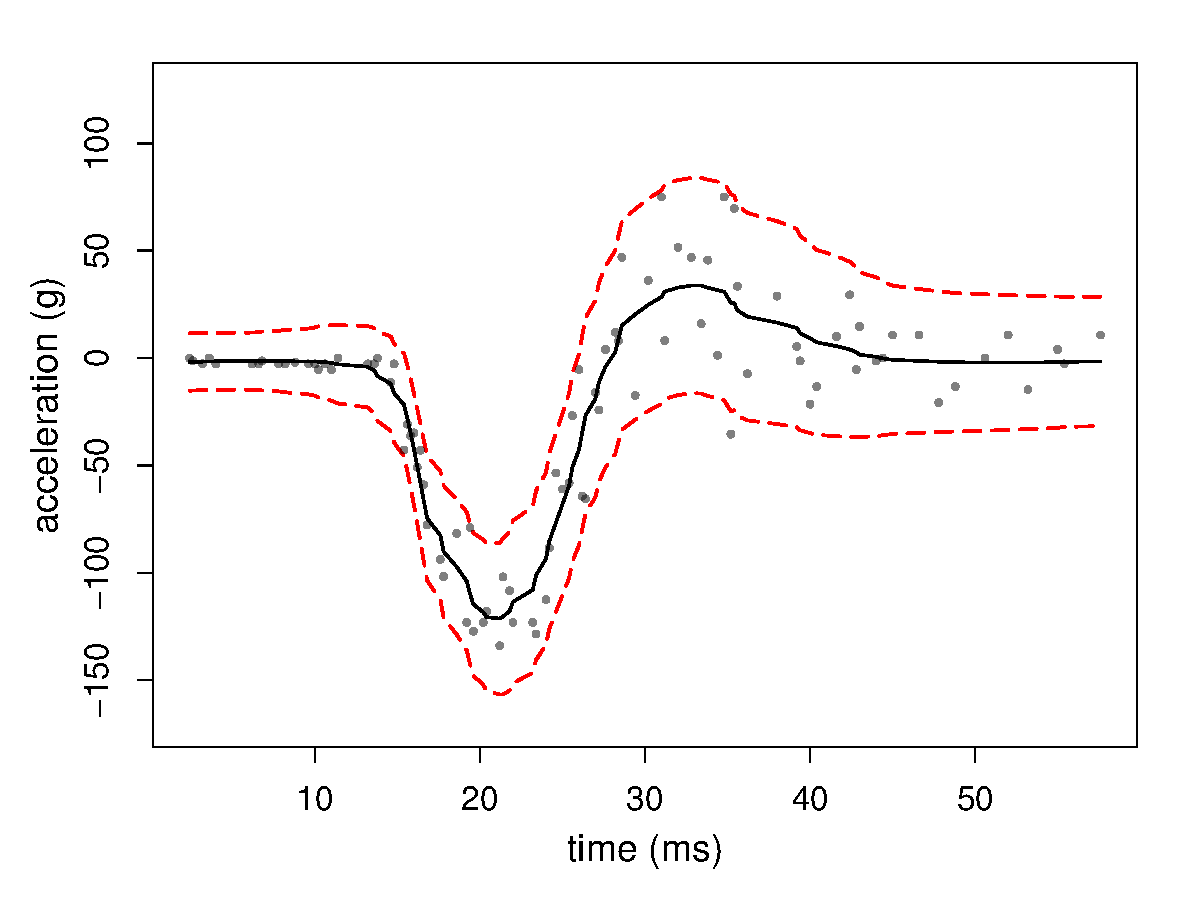
\includegraphics[width=0.65\textwidth]{motorcycle.pdf}
    \caption{Results from fitting SMASH to the motorcycle acceleration data discussed in \cite{silverman1985some}. The figure shows the estimate mean curve (solid black line) with $\pm2$ the estimated standard deviation curve (dashed red line).}
    \label{fig:motorcycle}
\end{figure}

As a further illustration of the heteroskedastic Gaussian version of SMASH, we apply it to the motorcycle acceleration dataset from \cite{silverman1985some}. The data consist of 133 observations measuring head acceleration in a simulated motorcycle accident that is used to test crash helmets. The dependent variable is {\it acceleration} (in {\it g}), and the independent variable is {\it time} (in {\it ms}). To deal with repeated measurements, we take the median of the measurements for acceleration for any given {\it time} value. As in Section \ref{sec:mfvb} we treat the 
data as if they are equally spaced although they are not. The fitted mean and variance curves (Figure \ref{fig:motorcycle})  
provide a visually appealing fit to the data, and were achieved without hand tuning of any parameters. This contrasts with
results in \cite{Delouille2004Smooth} -- which also uses a wavelet-based approach for heteroskedastic variance, but accounts for the unequal spacing of the data -- which required the {\it ad hoc} removal of high-resolution wavelet coefficients to produce a visual appealing fit.



%Although SMASH does a reasonably good job here, we recognize that there are better ways to deal with unequally spaced observations, which can 
%reveal the discontinuities in the first derivative around 15, 23 and 32 ms, as discussed in \cite{xx}. 


\subsection{ChIP-Seq Data}

To further illustrate our Poisson de-noising procedure we applied it to data from genomic sequencing. Specifically we applied SMASH to chromatin immunoprecipitation sequencing (ChIP-seq) data for the transcription factor {\it YY1} in cell line GM12878
collected by the ENCODE (\textbf{Enc}yclopedia \textbf{O}f \textbf{D}NA \textbf{E}lements) project. 
The data (e.g.~Figure \ref{fig:seq_peak_data}) consist of counts of sequencing reads mapping to each location in genome. These can be treated as
arising from an inhomogeneous Poisson process, whose intensity at base $b$ is related to the strength of the binding 
of the transcription factor near $b$. Because binding tends to be quite localized, the intensity is low on average (the vast majority of 
counts are 0), but has a small number of intense ``peaks". Identifying these peaks can help discover regions where 
binding occurs, which is an important component of understanding gene regulation. Consequently there are
many methods published for ``peak detection" in ChIP-Seq data \cite{Wilbanks2010Evaluation}. 

Our goal here is to outline how Poisson de-noising could provide an alternative approach to the analysis of ChIP-seq data.
The idea is simply to estimate the underlying intensity function, and then identify ``peaks" as regions where the estimated intensity
exceeds some threshold. 

To illustrate this idea we applied SMASH to ChIP-seq data from a region of length $2^{17} (\approx 131k)$ basepairs from chromosome 1
(hg19 chr1:880001-1011072). The estimated intensity is shown in Figure \ref{fig:seq_peak_est}, overlaid on peaks called by
the popular peak calling software MACS \cite{Zhang2008Modelbased}. We see that the locations with the strongest SMASH intensity estimates 
corresponds to peaks found by MACS.
However, the intensity estimate also suggests the presence of several additional weaker peaks not identified by MACS.

The reliable calling of peaks in ChIP-seq data is a multi-faceted problem, and a full assessment lies outside the scope of this paper.
Nonetheless, we believe that these illustrative results suggest that this approach could be worth pursuing further. 
One nice feature of the multi-scale poisson approach is that it deals well with a range of intensity functions, and could
perform well even in settings where peaks are broad and/or not especially well defined. In contrast, the performance of 
different peak-finding algorithms is often reported to be quite sensitive to the ``kinds" of peak
that are present, meaning that an algorithm that performs well in one setting may perform poorly in another.

%One advantage compared with many peak-calling approaches is that the method would provide an estimated intensity at every base-pair.

%Rather than calling peaks based on certain thresholds however, our method allows users to determine the relative strength and width of each peak, which provides a more comprehensive summary of the sequencing reads. At the same time, SMASH also provides the posterior variances for the intensity estimates, allowing for the option of calling peaks based on thresholds if desired.\\



%Since we are looking mainly at univariate denoising here, we ran our method on each sample separately to produce the the plots in Figure \ref{fig:seq_smooth}.\\
%\begin{figure}[h]
%\centering
%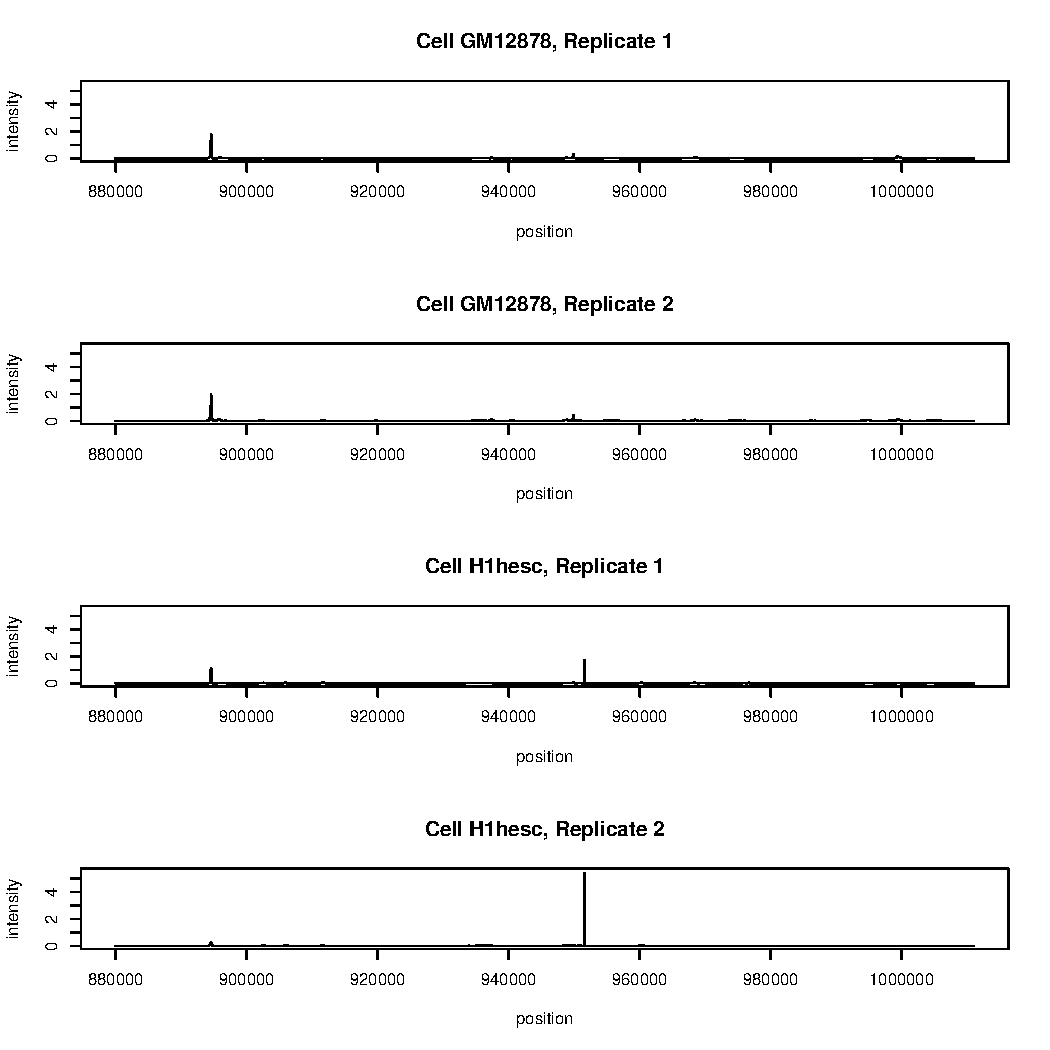
\includegraphics[scale=0.7]{smoothing_all.pdf}
%\caption{Estimated intensities from SMASH for 4 samples; the first two samples are two replicates from GM12878, a lymphoblastoid cell line, and the last two samples are two replicates from H1hesc, which are human embryonic stem cells. The reads are taken from position 880001 to 1011072 on chromosome 1.}
%\label{fig:seq_smooth}
%\end{figure}
%\bigskip
 
%In Figure \ref{fig:seq_smooth}, we immediately notice the presence of several large peaks around position 895000 for the first three samples, and around position 952000 for the last two samples.

\begin{figure}[p]
\centering
    \begin{subfigure}[b]{0.85\textwidth}
        \centering
        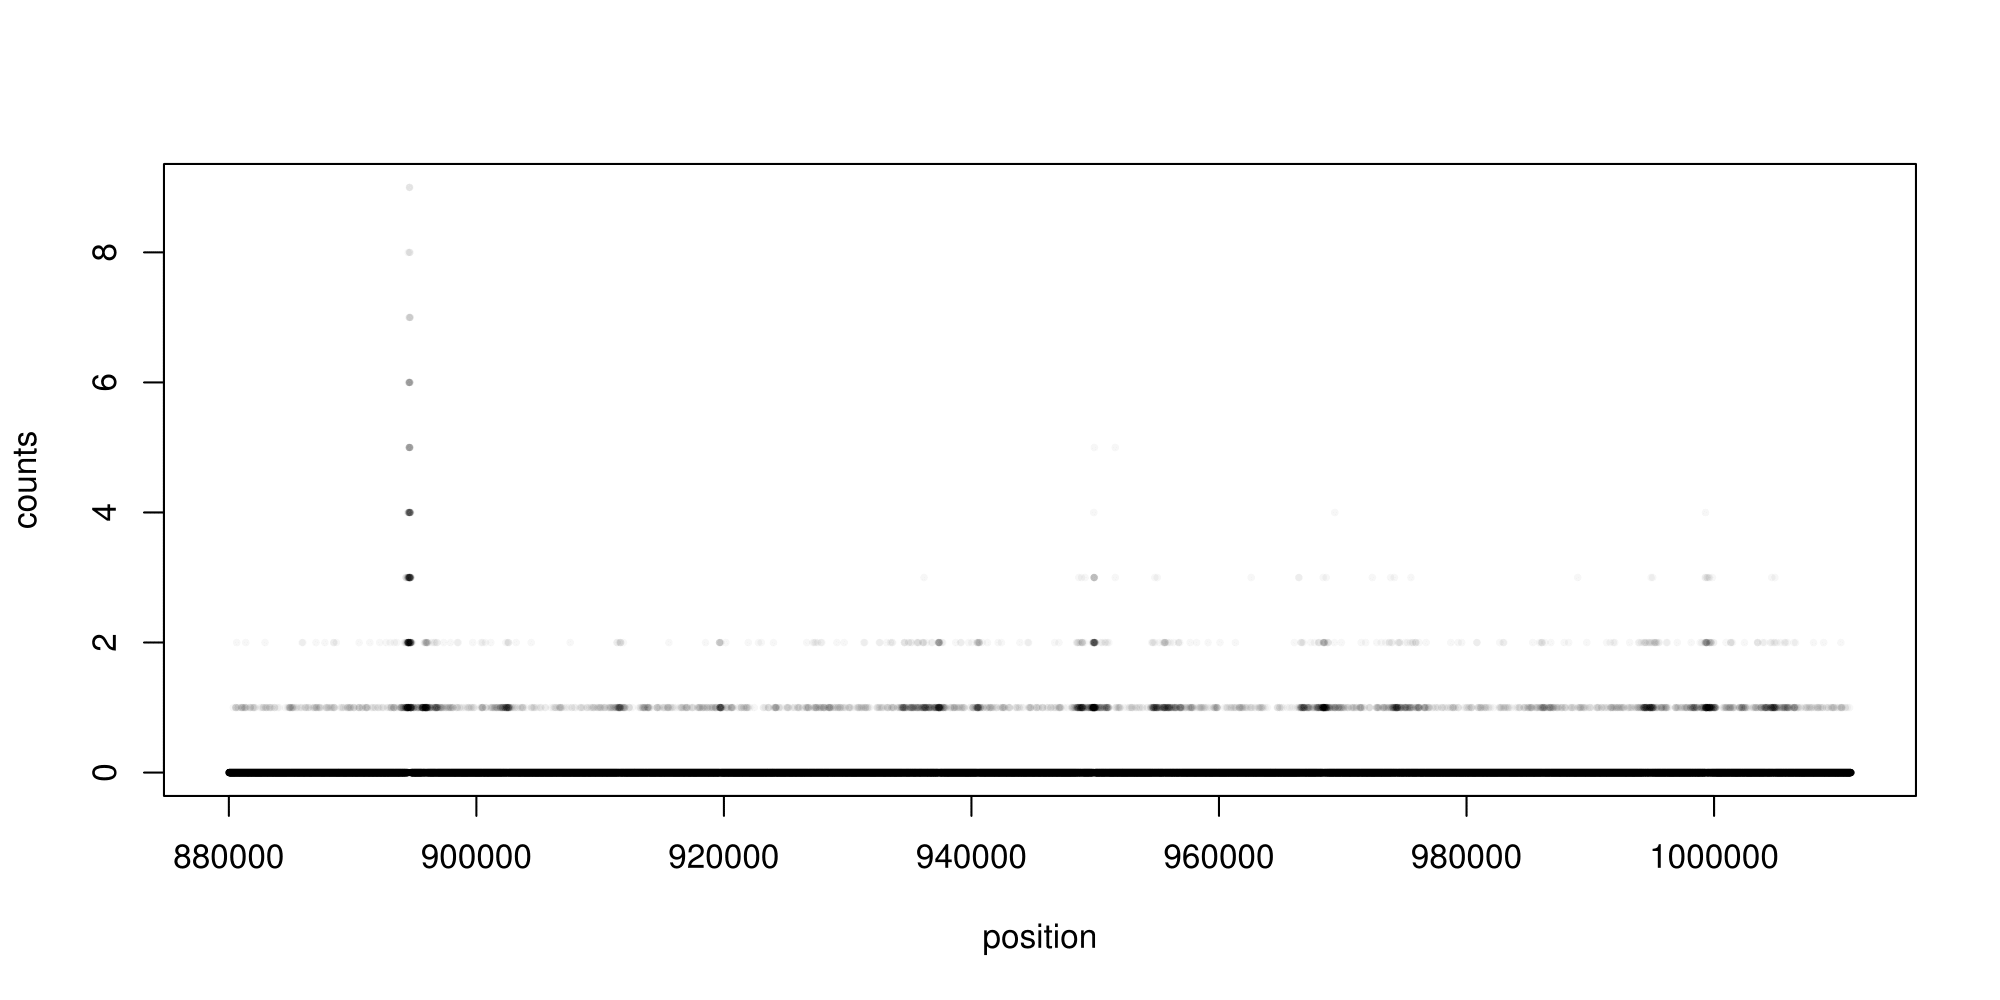
\includegraphics[width=\textwidth]{peaks_comp_a.png}
        \caption{}
        \label{fig:seq_peak_data}
    \end{subfigure}
    \begin{subfigure}[b]{0.85\textwidth}
        \centering
        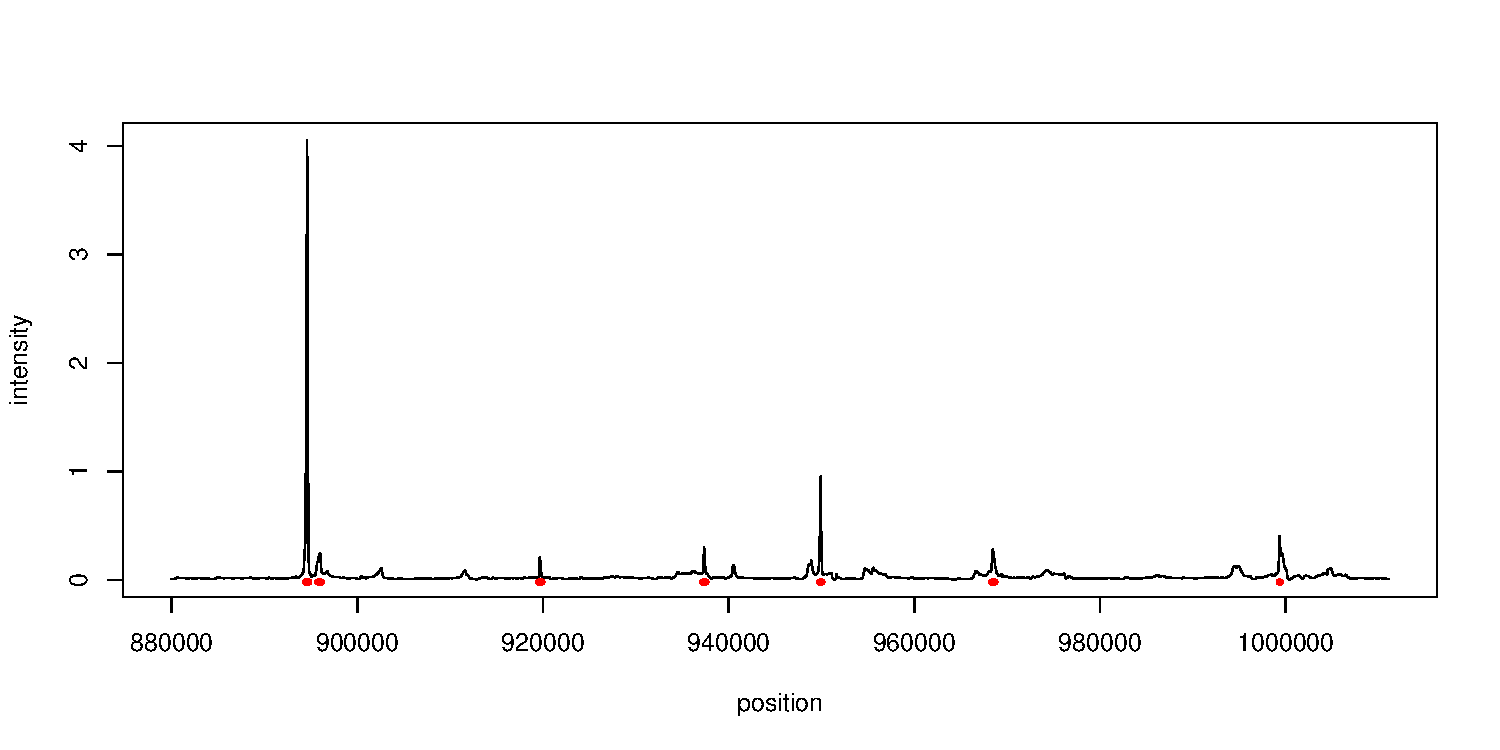
\includegraphics[width=\textwidth]{peaks_comp_b.pdf}
        \caption{}
        \label{fig:seq_peak_est}
    \end{subfigure}
    \caption{Illustration of how SMASH could be used to identify peaks in ChIP-seq data.  Panel (a) shows counts (summed across two replicate experiments). Due to over-plotting, darker regions of the plot correspond to higher concentrations of data points. Panel (b) shows the estimated intensity function from SMASH (black solid line) and location of peaks called by MACS (red markers beneath the estimated intensity).}
    \label{fig:seq_peak}
\end{figure}


\section{Discussion}

We have  adaptive shrinkage method ASH; while it was originally developed in the setting of FDR control for multiple comparisons, we have illustrated its usage as part of two wavelet denoising techniques. Both applications discussed in this paper relax the standard assumption of i.i.d. Gaussian noise, and are thus challenging tasks. Through these applications we are able to demonstrate the flexibility and accuracy of the shrinkage method, revealing its potential in many other applications.

First, our method provides a measure of uncertainty (through both the credible band for the mean curve as well as the variance curve itself), which is often of interest in many applications. 

In both the aforementioned applications, our software allows users to easily obtain point estimates for the mean function as well as their approximate posterior variances as a measure of uncertainty. In addition, the variance function can also be estimated, which would provide frequentist confidence intervals for other forms of mean estimation. To the best of our knowledge, there is no readily available software in the wavelet literature that implements joint mean and variance estimation. Simulations have also confirmed that our method is relatively robust to simple forms of autocorrelation between the errors (details needed). In the case of Poisson regression, we improved upon the conjugate Beta priors in \cite{Kolaczyk1999Bayesian} by using ASH as a shrinkage procedure, which allows for more flexibility and precision. %In addition, we have proposed a new procedure to assess the performance of a given method on real datasets without knowing the underlying truth, under the assumption that the data follow a Poisson distribution. 
In both the applications, one further advantage of both our methods is that there is no tuning parameter other than the type of wavelet basis used. On the other hand, the primary resolution level in almost all of the other wavelet-based methods actually affects their performance in varying degrees, depending on the underlying mean and/or variance function. Hence, our fully adaptive procedure allows users to easily apply it to any given dataset, depending on the type of noise.

potential to use likelihood to assess wavelet basis?

We have also demonstrated through numerical studies that our methods mostly outperform their respective counterparts from the standard wavelet literature, in terms of pointwise accuracy (MSE in this case). Furthermore, the simplicity of the approximated Gaussian likelihoods as well as the conjugacy of the mixture Gaussian priors imply that our methods are computationally fast, since the posteriors can be computed analytically. In the Gaussian case, simulation results demonstrated that our method is competitive with standard wavelet methods in the case of i.i.d. errors (without explicitly assuming thus), whilst maintaining superior accuracy when heteroskedastic errors are present. Unfortunately, the lack of readily available software (except for MFVB, as described in \cite{Menictas2015Variational}) for variance estimation made it difficult to assess the performance of our method in that context. On the other hand, we were able to compare our method to some of the more popular denoising techniques in the Poisson case. Specifically, we have improved upon the conjugate Beta priors used in conjunction with the binomial likelihoods \cite{Kolaczyk1999Bayesian}) by using ASH as the shrinkage procedure, which allows for more flexibility and accuracy. This is particularly evident when the mean intensity is low, as is common in many high-throughput genomic sequencing datasets. Our method is also much faster and comparable in accuracy to the popular Haar-Fisz algorithm. Unfortunately, we were not able to directly compare the computational efficiency of our method to many other methods due to differences in the programming software involved.

Although we focused on one-dimensional univariate denoising, our methods could be extended to more complex scenarios. In the one-dimensional domain, our methods could be used in conjunction with multiple samples, otherwise known as regression analysis of functional data (see \cite{Morris2006Waveletbased}). Instead of dealing with a vector of observations, we perform regression analysis on a matrix of observations, each row of which encapsulates a sample with temporally or spatially structured data points. While \cite{Morris2006Waveletbased} proposed a way to solve a generic regression model, they implicitly assumed the same variance structure for each sample in the same group or category. Our work in the Gaussian case potentially allows for differing variance structures amongst all the samples, thereby relaxing their assumptions. In the simplest case, we could obtain spatially structured differences between groups by including a single covariate that categorizes each sample. In particular, the Poisson model is extremely useful for discovering regions in sequencing reads where structured differences are present between say, various cell lines, as per our sequencing example in the previous section. The Gaussian model could potentially be used in...(??).

With some work, our methods could also be extended to higher dimensions, where a wider range of applications is possible. For example, we could attempt a straight extension to the two dimensional case for both the Gaussian and the Poisson cases as described in \cite{Nowak1999Multiscale}. However, recent research in image denoising problems has shown that discontinuities along edges present in many images such as photographs might render wavelet transformations undesirable \cite{Cande00}. We could thus incorporate ASH into other types of transformations such as curvelets \cite{Cande00}, which would be a potential direction for future work.
\newpage
\section{Reference}

\begin{appendices}
\section{}\label{app:var estimation}\bigskip
\textbf{Variance estimation for Gaussian denoising}


With $\bm{Z}$ as defined in \eqref{eq:varobs1}, we apply the wavelet transform $W$ to $\bm{Z}^2$, and obtain the wavelet coefficients $\bm{\Gd}=W\bm{Z}^2$. Note that $\mathbb{E}(\bm{\Gd})=(\bm{\Gg})$, where $\bm{\Gg}=W\bm{\s}^2$. Again we treat the likelihood for $\bm{\Gg}$ as if it were independent, resulting in
\begin{eqnarray}
L(\bm{\Gg}|\bm{\Gd})=\prod_{j=0}^J\prod_{k=0}^{T-1}P(\Gd_{jk}|\Gg_{jk})
\end{eqnarray}
However, the likelihoods $L(\Gg_{jk}|\Gd_{jk})$ are not normal, and have no simple closed form expressions. As such, we approximate the likelihood by a normal likelihood through matching the moments of a normal distribution to the distribution $P(\Gd_{jk}|\Gg_{jk})$ i.e.
\begin{eqnarray}
P(\Gd_{jk}|\Gg_{jk})\approx N(\Gg_{jk},\hat{\mathbb{V}}(\Gd_{jk}))
\end{eqnarray}
so that
\begin{eqnarray}\label{eq:gaus approx}
L(\Gg_{jk}|\Gd_{jk})\approx \phi(\Gd_{jk};\Gg_{jk},\mathbb{V}(\Gd_{jk}))
\end{eqnarray}
where $\phi$ is the normal density function, and $\mathbb{V}(\Gd_{jk})$ is the variance of the detail coefficients. Since these variances are unknown, we estimate them from the data and then proceed to treat them as known. More specifically, since $Z_t\sim N(0,\s_t^2)$, we have that
\begin{eqnarray}
&\mathbb{E}(Z_t^4)\approx 3\s_t^4\notag\\
\label{eq:varvarest}\Rightarrow&\mathbb{V}(Z_t^2)\approx 2\s_t^4
\end{eqnarray}
and so we simply use $\frac{2}{3}Z_t^4$ as an unbiased estimator for $\mathbb{V}(Z_t^2)$. It then follows that $\hat{\mathbb{V}}(\Gd_{jk})$ is given by $\sum_{l=1}^n \frac{2}{3}Z_l^4W_{jk,l}^2$, and is unbiased for $\mathbb{V}(\Gd_{jk})$. These will be the inputs to ASH, which then produces shrunk estimates in the form of posterior means for the corresponding parameters. Although this works well in most cases, there are variance functions for which the above procedure tends to overshrink the wavelet coefficients at the finer levels. This is likely because the distribution of the wavelet coefficients is extremely skewed, especially when the true coefficients are small (at coarser levels the distributions are much less skewed since we are dealing a linear combination of a large number of data points). One way around this issue is to employ a procedure that jointly shrinks the coefficients $\bm{\Gg}$ and their variance estimates (see JASH). The final estimate of the variance function is obtained from the posterior means via the average basis inverse across all the shifts.

\section{}\label{app:reconstruction}\bigskip
\textbf{Poisson denoising}

First summarize the data in a recursive manner: 
\begin{eqnarray}
Y_{Jk}\equiv Y_k\end{eqnarray}
for $k=1,...,n$, and
\begin{eqnarray}
Y_{jk}=Y_{j+1,2k}+Y_{j+1,2k+1}
\end{eqnarray}
for resolution $j=0,...,J-1$ and location $k=0,...,2^j-1$. Hence, we are summing more blocks of observations as we move to coarser levels. 

This recursive scheme leads to:
\begin{eqnarray}
Y_{jk}=\sum_{l=k2^{J-j}+1}^{(k+1)2^{J-j}}Y_l
\end{eqnarray}
for $j=0,...,J$ and $k=0,...,2^j-1$.

Further define the following:
\begin{eqnarray}\Gl_{Jk}\equiv \Gl_k\end{eqnarray}
for $k=1,...,n$, and
\begin{eqnarray}\Gl_{jk}=\Gl_{j+1,2k}+\Gl_{j+1,2k+1}\end{eqnarray}
for $j=0,...,J-1$ and $k=0,...,2^j-1$. 
Furthermore, define
\begin{eqnarray}\label{eq:poisson wc}\Ga_{jk}=\log(\Gl_{j+1,2k})-\log(\Gl_{j+1,2k+1})\\\end{eqnarray}
for $s=0,...,J-1$ and $l=0,...,2^j-1$. The ${\Ga}$'s defined this way is extremely similar to the (true) Haar wavelet coefficients, which forms the basis of our approach. Using this recursive representation, we can see that the likelihood for $\bm{\Ga}$ factorizes into a product of likelihoods, where $\bm{\Ga}$ is the vector of all the $\Ga_{sl}$'s. To be specific, we have
\begin{eqnarray}
L(\bm{\Ga}|\mathbf{Y})&=&P(\mathbf{Y}|\bm{\Ga})\\
&=&P(Y_{0,0}|\Gl_{0,0})\prod_{j=0}^{J-1}\prod_{k=0}^{2^j-1}P(Y_{j+1,2k}|Y_{j,k},\Ga_{j,k})\\
&=&L(\Gl_{0,0}|Y_{0,0})\prod_{j=0}^{J-1}\prod_{k=0}^{2^j-1}L(\Ga_{j,k}|Y_{j+1,2k},Y_{j,k})
\end{eqnarray}
where the factorization is due to the recursive definition above. Note that $Y_{00}|\Gl_{00}\sim \textrm{Pois}(\Gl_{00})$. For any given $j,k$, $Y_{jk}$ is a sum of two independent Poisson random variables, and is itself a Poisson random variable. Hence
\[Y_{j+1,2k}|Y_{jk},\Ga_{jk}\sim \textrm{Bin}({Y_{jk},\frac{1}{1+e^{-\Ga_{jk}}}\equiv\frac{\Gl_{j+1,2k}}{\Gl_{jk}}})\]

\subsection{Estimates and standard errors for $\alpha_j$}

Each $\alpha_{j}$ is a ratio of the form $\log(\mu_{a:b}/\mu_{c:d})$ whose maximum likelihood estimate (mle) is $\log(Y_{a:b}/Y_{c:d})$. The main challenge here is that the mle is not well behaved when either the numerator or denominator of $Y_{a:b}/Y_{c:d}$ is 0. To deal with this, when either is 0 we use Tukey's modification \cite{Gart1967Bias}. Specifically, letting $S$ denote $Y_{a:b}$ and $F$ denote $Y_{c:d}$ (corresponding to thinking of these as successes and failures in a binomial experiment, given $Y_{a:b}+Y_{c:d}$), we use
\begin{eqnarray}\label{eq:pseudoMLE1}
&&\hat{\Ga}=\left\{
\begin{array}{lll}
\log\{(S+0.5)/(F+0.5)\}-0.5&\ \ \ S=0\\
\log\{S/F\}&\ \ \ S=1,2,...,N-1\\
\log\{(S+0.5)/(F+0.5)\}+0.5&\ \ \ S=N\\
\end{array}
\right.\\ \label{eq:pseudoMLE1se}
&&se(\hat{\Ga})=\sqrt{V^*(\hat{\Ga})-\frac{1}{2}\{V_3(\hat{\Ga})\}^2\left\{V_3(\hat{\Ga})-\frac{4}{N}\right\}}
\end{eqnarray}
where
\begin{eqnarray}
&&V_3(\hat{\Ga})=\frac{N+1}{N}\left(\frac{1}{S+1}+\frac{1}{F+1}\right)\ \ \ S=0,...,N\\
\label{eq:pseudoMLE2}&&V^*(\hat{\Ga})=V_3(\hat{\Ga})\left\{1-\frac{2}{N}+\frac{V_3(\hat{\Ga})}{2}\right\}
\end{eqnarray}
The square of the standard error in \eqref{eq:pseudoMLE1se} corresponds to $V^{\ast\ast}$ from p. 182 of \cite{Gart1967Bias}, and is chosen because it is less biased for the true variance of $\hat{\Ga}$ (when $N$ is small) as compared to the asymptotic variance of the MLE (see \cite{Gart1967Bias}). The other two variance estimators from \cite{Gart1967Bias}, $V_1^{++}$ and $V^{++}$, were also considered in simulations and gave similar results, but $V^{\ast\ast}$ was chosen for its simple form.


%One direct approximation of the likelihood for $\Ga$ is the Laplace approximation, which results in the Gaussian likelihood given by $\phi(\Ga;\hat{\Ga}_{MLE},\mathbb{V}(\hat{\Ga}_{MLE}))$. Here $\phi$ is the normal density function, and $\hat{\Ga}_{MLE}$ is the maximum likelihood estimator. We would then estimate $\mathbb{V}(\hat{\Ga}_{MLE})$ by the square of the asymptotic standard deviation for $\hat{\Ga}_{MLE}$. Specifically,
% for some appropriate estimator $\hat{\Ga}$. This choice of parameters for the Gaussian approximation is also appropriate in the sense that it minimizes the Kullback-Leibler divergence between a Gaussian distribution and the likelihood for $\Ga$ (also known as moment matching).

%We next consider appropriate estimators for the parameters $\Ga$ and $\sqrt{\mathbb{V}(\hat{\Ga})}$. The obvious choice would be the MLE of $\Ga$ and its asymptotic standard error respectively, given by
%\begin{eqnarray}
%\hat{\Ga}_{MLE}=\log(S/F)&\ \ \ S=0,...,N\\
%se(\hat{\Ga}_{MLE})=\sqrt{SF/N}&\ \ \ S=0,...,N
%\end{eqnarray}
%where $S$ is the number of successes in the binomial setup, and $F=N-S$ is the number of failures (in our case the even locations would be successes and odd locations failures). The MLE has one notable drawback however, in that it cannot deal well with extreme cases. This would in turn affect the likelihood approximation in a non-negligible way. To improve the accuracy of the approximation at the endpoints of the binomial distribution (ie. when we have $\hat{p}=0$ or $N$, so that $\hat{\Ga}=-\infty$ or $\infty$ respectively), we instead aim to find a suitable estimator $\hat{\Ga}$ for $\Ga$. Next, we approximate the distribution of $\hat{\Ga}$ by a Gaussian distribution, so that the likelihood for $\Ga$ is automatically Gaussian, given by $\phi(\Ga;\hat{\Ga},\mathbb{V}(\hat{\Ga}))$. 

\subsection{Signal reconstruction}

Given the posterior means and variances of the $\Ga$'s from ASH, the first step to reconstructing the signal is to find the posterior means of $p_{jk}:=\frac{\Gl_{j+1,2k}}{\Gl_{jk}}$ and $q_{jk}:=\frac{\Gl_{j+1,2k+1}}{\Gl_{jk}}$ (for $j=0,...,J-1$ and $k=0,...,2^j-1$). Specifically, for each $j$ and $k$, we wish to find
\begin{eqnarray}\label{eq:pfromwc1}
&&E(p_{jk})\equiv E\left(\frac{e^{\Ga_{jk}}}{1+e^{\Ga_{jk}}}\right)\\
\label{eq:pfromwc2}&&E(q_{jk})\equiv E\left(\frac{e^{-\Ga_{jk}}}{1+e^{-\Ga_{jk}}}\right)\end{eqnarray}
Given that we already have the posterior expectations and variances for $\Ga_{jk}$, we can approximate \eqref{eq:pfromwc1}-\eqref{eq:pfromwc2} using the Delta method. First, define
\begin{eqnarray}\label{eq:ff}ff(x)=\frac{e^x}{1+e^x}\end{eqnarray}
and consider the Taylor expansion of $ff(x)$ about $ff(E(x))$:
\begin{eqnarray}\label{eq:delta}ff(x)\approx ff(E(x))+ff'(E(x))(x-E(x))+\frac{ff''(E(x))}{2}(x-E(x))^2\end{eqnarray}
where
\begin{eqnarray}
\label{eq:fderiv}&&ff'(x)=\frac{e^x}{(1+e^x)^2}\\
\label{eq:sderiv}&&ff''(x)=\frac{e^x(1-e^{x})}{(1+e^x)^3}
\end{eqnarray}
It is easy to see that
\begin{eqnarray}
&&E(p_{jk})\approx ff(E(\Ga_{jk}))+\frac{ff''(E(\Ga_{jk}))}{2}Var(\Ga_{jk})\\
\label{eq:Ep}&&E(q_{jk})\approx ff(-E(\Ga_{jk}))+\frac{ff''(-E(\Ga_{jk}))}{2}Var(\Ga_{jk})
\end{eqnarray}
noting that we have already computed $E(\Ga)$ and $Var(\Ga)$.

Finally, we can easily back-transform to construct an estimated signal, by noting that we can express $\Gl_t$ as a product of the $p$'s and $q$'s for any $i=1,2,...,n$. Specifically, let $\{c_1,...,c_J\}$ be the binary representation of $i-1$, and $d_m=\sum_{j=1}^m c_j2^{m-j}$ for $j=1,...,J-1$. We then have
\begin{eqnarray}\label{eq:product}\Gl_k=\Gl_{00}p_{00}^{1-c_1}p_{1,d_1}^{1-c_2}...p_{J-1,d_{J-1}}^{1-c_J}q_{00}^{c_1}q_{1,d_1}^{c_2}...q_{J-1,d_{J-1}}^{c_J}\end{eqnarray}
where we usually estimate $\Gl_{00}$ by $\sum_l Y_l$ (see Kolaczyk (1999)). Using the independence of the $p$'s and $q$'s from different scales, we have:
\begin{eqnarray}\label{eq:Eproduct}E(\Gl_t)=\Gl_{00}E(p_{00})^{1-c_1}E(p_{1,d_1})^{1-c_2}...E(p_{J-1,d_{J-1}})^{1-c_J}\notag\\
E(q_{00})^{c_1}E(q_{1,d_1})^{c_2}...E(q_{J-1,d_{J-1}})^{c_J}\end{eqnarray}

As an additional step, we can also construct a credible band around the signal using the posterior variances for inference purposes. From \eqref{eq:product} we have the following:
\begin{eqnarray}\label{eq:E2product}E(\Gl_t^2)=\Gl_{00}^2E(p_{00}^2)^{1-c_1}E(p_{1,d_1}^2)^{1-c_2}...E(p_{J-1,d_{J-1}}^2)^{1-c_J}\notag\\
E(q_{00}^2)^{c_1}E(q_{1,d_1}^2)^{c_2}...E(q_{J-1,d_{J-1}}^2)^{c_J}\end{eqnarray}
To compute the terms in \eqref{eq:E2product}, we again make use of the Delta method (with $ff(x)=(\frac{e^x}{1+e^x})^2$) to obtain:
\begin{eqnarray}
&E(p_{jk}^2)\approx \left(ff(E(\Ga_{jk}))+\frac{ff''(E(\Ga_{jk}))}{2}Var(\Ga_{jk})\right)^2+\notag\\
& \hspace{1.5 in}\{ff'(E(\Ga_{jk}))\}^2Var(\Ga_{jk})\\
&E(q_{jk}^2)\approx \left(ff(-E(\Ga_{jk}))+\frac{ff''(-E(\Ga_{jk}))}{2}Var(\Ga_{jk})\right)^2+\notag\\
& \hspace{1.5 in}\{ff'(E(-\Ga_{jk}))\}^2Var(\Ga_{jk})
\end{eqnarray}
Finally we combine \eqref{eq:Eproduct} and \eqref{eq:E2product} to find $Var(\Gl_k)$, which allows us to construct credible intervals.

Note here that for the reconstructed signal to possess the property of shift invariance (\cite{Coifman1995Translationinvariant}), the $\Ga$'s are extracted from a so-called translation invariant (TI) table (see \cite{Coifman1995Translationinvariant}, and \cite{Kolaczyk1999Bayesian}) rather than as described above. The idea remains the same however, and we can simply think of the extra $\Ga$'s as being defined similarly as the original $\Ga$'s, albeit from a shifted version of the original data points. To be more specific, the TI table contains the $\Ga_{jk}$ for all circulant shifts of the signal. Here we define the $t$-th shift of the signal $\bm{Y}$, denoted by $\bm{Y}^{(t)}$, to be created from $\bm{Y}$ itself by moving the first $n-t$ elements of $\bm{Y}$ $t$ positions to the right and then putting the last $t$ elements of $\bm{Y}$ in the first $t$ locations. Using this table, we are essentially computing the posterior expectations in \eqref{eq:Eproduct}-\eqref{eq:E2product} by averaging over all posterior expectations for every shift of the original signal ie.
\begin{eqnarray}
\label{eq:TIapproxexp}\frac{1}{n}\sum_{t=1}^n E(\hat{\Gl}_k^{(t)})
\end{eqnarray}
which is an approximation to the true quantity we wish to compute, given by
\begin{eqnarray}
E(\hat{\Gl}_k)=\sum_{t=1}^n E(\hat{\Gl}_k^{(t)})P(\mbox{$t$-th shift})
\end{eqnarray}
\end{appendices}

\bibliography{smash}
\bibliographystyle{plain}

\end{document}
